%%%%%%%%%%%%%%%%%%%%%%%%%%%%%%%%%%%%%%%%%%%%%%%%%%%%%%%%%%%%%%%%%%%%
%%%%%%%%%%%%%%%%%%%%%%%%%%%%%%%%%%%%%%%%%%%%%%%%%%%%%%%%%%%%%%%%%%%%
%%                                                                %%
%% An example for writting your thesis using LaTeX                %%
%% Original version by Luis Costa,  changes by Perttu Puska       %%
%% Support for Swedish added 15092014                             %%
%%                                                                %%
%% This example consists of the files                             %%
%%         thesistemplate.tex (versio 2.01)                       %%
%%         opinnaytepohja.tex (versio 2.01) (for text in Finnish) %%
%%         aaltothesis.cls (versio 2.01)                          %%
%%         kuva1.eps                                              %%
%%         kuva2.eps                                              %%
%%         kuva1.pdf                                              %%
%%         kuva2.pdf                                              %%
%%                                                                %%
%%                                                                %%
%% Typeset either with                                            %%
%% latex:                                                         %%
%%             $ latex opinnaytepohja                             %%
%%             $ latex opinnaytepohja                             %%
%%                                                                %%
%%   Result is the file opinnayte.dvi, which                      %%
%%   is converted to ps format as follows:                        %%
%%                                                                %%
%%             $ dvips opinnaytepohja -o                          %%
%%                                                                %%
%%   and then to pdf as follows:                                  %%
%%                                                                %%
%%             $ ps2pdf opinnaytepohja.ps                         %%
%%                                                                %%
%% Or                                                             %%
%% pdflatex:                                                      %%
%%             $ pdflatex opinnaytepohja                          %%
%%             $ pdflatex opinnaytepohja                          %%
%%                                                                %%
%%   Result is the file opinnaytepohja.pdf                        %%
%%                                                                %%
%% Explanatory comments in this example begin with                %%
%% the characters %%, and changes that the user can make          %%
%% with the character %                                           %%
%%                                                                %%
%%%%%%%%%%%%%%%%%%%%%%%%%%%%%%%%%%%%%%%%%%%%%%%%%%%%%%%%%%%%%%%%%%%%
%%%%%%%%%%%%%%%%%%%%%%%%%%%%%%%%%%%%%%%%%%%%%%%%%%%%%%%%%%%%%%%%%%%%

%% Uncomment one of these:
%% the 1st when using pdflatex, which directly typesets your document in
%% pdf (use jpg or pdf figures), or
%% the 2nd when producing a ps file (use eps figures, don't use ps figures!).
\documentclass[english,12pt,a4paper,pdftex,sci,utf8]{aaltothesis}
%\documentclass[english,12pt,a4paper,dvips]{aaltothesis}
\linespread{1.05}

%% To the \documentclass above
%% specify your school: arts, biz, chem, elec, eng, sci
%% specify the character encoding scheme used by your editor: utf8, latin1

\usepackage{graphicx}

%% Use this if you write hard core mathematics, these are usually needed
\usepackage{amsfonts,amssymb,amsbsy}

\usepackage{paralist}
\usepackage{algorithm}
\usepackage{algpseudocode}
\usepackage{listings}


%% Use the macros in this package to change how the hyperref package below 
%% typesets its hypertext -- hyperlink colour, font, etc. See the package
%% documentation. It also defines the \url macro, so use the package when 
%% not using the hyperref package.
%%
%\usepackage{url}

%% Use this if you want to get links and nice output. Works well with pdflatex.
\usepackage{hyperref}
\hypersetup{pdfpagemode=UseNone, pdfstartview=FitH,
  colorlinks=true,urlcolor=red,linkcolor=blue,citecolor=black,
  pdftitle={LenticularFS: scalable filesystem for the cloud},
  pdfauthor={Roberto Bampi}, pdfkeywords={HDFS, filesystem}}
  
\setlength{\abovecaptionskip}{15pt plus 3pt minus 2pt} % Chosen fairly arbitrarily
\setlength{\belowcaptionskip}{15pt plus 3pt minus 2pt} % Chosen fairly arbitrarily

\lstset{
    language=Java,
    basicstyle=\small\ttfamily,
    keywordstyle=\color{blue}\ttfamily,
    stringstyle=\color{red}\ttfamily,
    commentstyle=\color{green}\ttfamily,
    morecomment=[l][\color{magenta}]{\#},
    numbers=left,
    showspaces=false,
    showstringspaces=false,
    frame=L,
}

%% All that is printed on paper starts here
\begin{document}
\renewcommand{\thesissupervisorname}{Thesis supervisors}



%% Change the school field to specify your school if the automatically 
%% set name is wrong
% \university{aalto-yliopisto}
% \university{aalto University}
% \school{Sähkötekniikan korkeakoulu}
% \school{School of Electrical Engineering}

%% Only for B.Sc. thesis: Choose your degree programme. 
%\degreeprogram{Electronics and electrical engineering}
%%

%% ONLY FOR M.Sc. AND LICENTIATE THESIS: Specify your department,
%% professorship and professorship code. 
%%
\department{Department of Computer Science}
%% \professorship{Circuit theory}
%%

\univdegree{MSc}

%% Your own name (should be self explanatory...)
\author{Roberto Bampi}

%% Your thesis title comes here and again before a possible abstract in
%% Finnish or Swedish . If the title is very long and latex does an
%% unsatisfactory job of breaking the lines, you will have to force a
%% linebreak with the \\ control character. 
%% Do not hyphenate titles.
%% 
\thesistitle{LenticularFS: Scalable filesystem for the cloud}

\place{Kista}

%% For B.Sc. thesis use the date when you present your thesis. 
%% 
%% Kandidaatintyön päivämäärä on sen esityspäivämäärä! 
\date{14.9.2017}

%% B.Sc. or M.Sc. thesis supervisor 
%% Note the "\" after the comma. This forces the following space to be 
%% a normal interword space, not the space that starts a new sentence. 
%% This is done because the fullstop isn't the end of the sentence that
%% should be followed by a slightly longer space but is to be followed
%% by a regular space.
%%
% \supervisor{Prof.\ Jim Dowling} %{Prof.\ Pirjo Professori}
\supervisor{Prof.\ Keijo Heljanko}
%% B.Sc. or M.Sc. thesis advisors(s). You can give upto two advisors in
%% this template. Check with your supervisor how many official advisors
%% you can have.
%%
\advisor{Prof.\ Jim Dowling}
% \advisor{D.Sc.\ }
% \advisor{M.Sc.\ }

%% Aalto logo: syntax:
%% \uselogo{aaltoRed|aaltoBlue|aaltoYellow|aaltoGray|aaltoGrayScale}{?|!|''}
%%
%% Logo language is set to be the same as the document language.
%% Logon kieli on sama kuin dokumentin kieli
%%
\uselogo{aaltoRed}{''}

%% Create the coverpage
%%
\makecoverpage


%% Note that when writting your master's thesis in English, place
%% the English abstract first followed by the possible Finnish abstract
%% English abstract.
%% All the information required in the abstract (your name, thesis title, etc.)
%% is used as specified above.
%% Specify keywords
%%
%% Kaikki tiivistelmässä tarvittava tieto (nimesi, työnnimi, jne.) käytetään
%% niin kuin se on yllä määritelty.
%% Avainsanat
%%
\keywords{}
%% Abstract text
\begin{abstractpage}[english]

The Hadoop platform is the most common solution to handle the explosion of big-data that both companies and research institutions are facing.
In order to store such data, the Hadoop platform provides HDFS, a scalable distributed filesystem which runs on commodity hardware and enables linear scalability by adding new storage nodes.
While storage capacity of the system can be increased by adding new storage nodes, the component that handles metadata for the filesystem, the namenode, is a single point of failure and cannot easily replaced or linearly scaled.
The Hops projects provides an alternative implementation of the namenode, which increases performance and scalability by storing metadata on an external distributed NewSQL database called MySQL Cluster.
With the new architecture, the system is much more scalable and can transparently manage the failover of namenodes which are now stateless components.
HopsFS is, however, still limited to running within a single datacenter which can cause severe outages in case the entire datacenter becomes unavailable.
Cloud native storage systems, such as Amazon's Simple Storage Service (S3), solve this problem by replicating data across different, geographically distant datacenters, so that the failure of any given zone does not cause data unavailability.
The objective of this thesis is to enable HopsFS to work across geographical regions while, as far as possible, maintaining the semantics of a POSIX-style hierarchical filesystem.
We leverage asynchronous replication functionality provided by MySQL Cluster to obtain replication of metadata across geographical regions and we present a detailed analysis on how to maintain the consistency properties of HDFS in such an environment.
Furthermore, we analyze the issue of split brain scenarios and propose a way for namenodes to detect this condition and continue operating correctly.
Finally, we discuss the changes to the codebase which are required to implement the proposed plan.


\end{abstractpage}

%% Force a new page so that the possible English abstract starts on a new page
%%
%% Pakotetaan uusi sivu varmuuden vuoksi, jotta 
%% mahdollinen suomenkielinen ja englanninkielinen tiivistelmä
%% eivät tule vahingossakaan samalle sivulle
\newpage
%
%% Abstract in Finnish.  Delete if you don't need it. 
%% Preface
%%
%% Esipuhe 
\mysection{Preface}
%\mysection{Esipuhe}
% I want to thank Professor Pirjo Professori
% and my instructor Olli Ohjaaja for their 
% good and poor guidance.\\

\vspace{5cm}
Trento, 12.9.2017

\vspace{5mm}
{\hfill Roberto Bampi \hspace{1cm}}

%% Force new page after preface
%%
%% Pakotetaan varmuuden vuoksi esipuheen jälkeinen osa
%% alkamaan uudelta sivulta
\newpage


%% Table of contents. 
\thesistableofcontents


%% Tweaks the page numbering to meet the requirement of the thesis format:
%% Begin the pagenumbering in Arabian numerals (and leave the first page
%% of the text body empty, see \thispagestyle{empty} below).
%% Additionally, force the actual text to begin on a new page with the 
%% \clearpage command.
%% \clearpage is similar to \newpage, but it also flushes the floats (figures
%% and tables).
%% There is no need to change these
%%
\cleardoublepage
\storeinipagenumber
\pagenumbering{arabic}
\setcounter{page}{1}

\section{Introduction}
\label{section:intro}

%% Leave first page empty
\thispagestyle{empty}

\footnote{TODO: intro to big data, http://queue.acm.org/detail.cfm?id=1594206}
The Apache Hadoop project is by far the most well-known open source toolkit for the storage and processing of big data.
Since its inception, the Hadoop project moved from a map-reduce framework to a generic set of loosely coupled services that can be used for many different kinds of computation.
One of the most important components of this ecosystem and the focus of this thesis is HDFS.

Apache HDFS is a distributed filesystem designed to store very large files and allow for programs and frameworks written in different languages to operate on the data.
It is successfully deployed by many companies and it is capable of running on very large clusters.
Its design uses a single node, the namenode, to centrally manage metadata for the whole cluster and this creates a limitation for both the scalability and robustness as the system as a whole.
To improve robustness it is possible to run a second namenode which will act as a hot-standby, ready to replace the primary in case of problems, and then either trigger a manual failover or configure the cluster for automatic failover using Zookeeper.
While both methods improve the reliability of the system, neither does so without significant complications.
First, both methods require the cluster operator to run additional services, the JournalNodes, just to keep the standby namenode in sync with the primary.
In case of manual failover, the cluster operator must then manually verify and trigger the operation in case of problems, which is a slow and error prone procedure.
In case of automatic failover, however, the cluster operator is required to configure and manage a Zookeeper cluster and a ZKFailoverController process on every namenode which significantly increases the complexity of the deployment as a whole.
Furthermore neither solution improves the scalability of the system because all RPCs are still directed to the active namenode.

The limitations described also present challenges for operators that want to run their HDFS clusters in public cloud environments such as Amazon Web Services (AWS), Google Cloud Platform (GCP) or Microsoft Azure.
Public clouds offer virtual machines that are executed on hypervisors that are shared with other customers, and performance and reliability tend to be unpredictable as a result.
Cloud provider also tend to provide reliability at a more abstract level than on-premise deployments.
Whereas in a typical data-center the failure domains are machine, rack, and whole data-center, cloud providers have machines, availability zones and regions.
Single instances in most cloud providers are considered unreliable and expendable, therefore proper cloud software should be resilient to the failure of any one instance by distributing or replicating processes onto multiple instances.
HDFS expectation that the machine hosting the namenode be stable and with consistent performance is therefore difficult to achieve in cloud environments, even when considering an high availability setup.
To solve this problem, most providers offer managed offers of Hadoop that can automatically create and manage clusters and let the customer focus on writing the data processing pipeline.
This does not, however, solve the problem of efficiently managing HDFS clusters in the cloud.

To store large amount of data on the cloud, the most popular approach is to use provider-managed cloud storage solutions such as Amazon's Simple Storage Service (S3), Google Cloud Storage or Azure Blob storage.
These systems allow customers to use a simple API to upload, list, and retrieve millions of blobs which can be several terabytes in size each.
Furthermore these services seamlessly scale without any user intervention and are priced according to the amount of data consumed and the bandwidth used to operate on them.
While it may sound tempting to adapt applications to use cloud storage systems and forego HDFS, and hierarchical filesystems entirely, these system do not offer the primitives associated with traditional (distributed) filesystems.
First, these systems are actually key-value stores that associate a key, the path name, to a value, the blob.
While this helps with scalability, different keys can be mapped to different storage machines, it makes common operations such as listing the content of directories much slower and with a linear time increase with the number of entries in the store. 
Furthermore, to maintain their favourable scalability characteristics and fault-tolerance, they sacrifice consistency for availability in the face of network partitions, resulting in an eventually consistent system.
Eventually consistent systems propagate changes in the system asynchronously which may result in client retrieving stale data, such as a listing of a directory missing some newly created files or a payload fetch which still retrieves a recently deleted object.
To allow these systems to offer consistency semantics equal to those of HDFS, some cloud providers, such as Amazon for their managed Hadoop offer (EMR), build additional software that expose a HDFS-compliant API while managing metadata in such a way that the overall system appears to have consistent metadata.
The trade-offs are that this approach introduces further components that need to be managed and scaled, it worsens performance of the overall system because of the wait times required for the changes to propagate through the system, and it introduces the possibility of the metadata store becoming inconsistent with the underlying data store.

To solve the mismatch of HDFS with cloud environments, the Hops project provides a scalable, cloud-ready, protocol-compatible distribution of HDFS called HopsFS \cite{DBLP:conf/dais/NiaziIBD15}.
HopsFS solves the biggest architectural problem that limits both HDFS's scalability and its fault-tolerance, the storage of filesystem metadata in the namenode process main memory.
Unlike HDFS, HopsFS stores the metadata in a distributed, consistent NewSQL database called Mysql Cluster, which can scale to hundreds of machines and store hundreds of terabytes of metadata.
By moving the metadata in an external component, the namenode effectively becomes a (mostly) stateless process which can be easily replicated on multiple machines, all connecting to the same metadata storage cluster.
Aside from a clear improvement in availability, all of the HopsFS datanodes can answer RPC requests traditionally directed towards the HDFS namenode, enabling horizontal scalability at the namenode layer.
As demonstrated in \cite{DBLP:conf/dais/NiaziIBD15} on a workload trace provided by Spotify, the improvements brought by the increased scalability allow HopsFS to perform 16 times the number of metadata operations in the same amount of time.
Furthermore, the filesystem metadata is now accessible to other applications in a transactional SQL database, allowing other programs to consume and extend the model for their own purposes.
% aggiungi citazione a buso qui

While HopsFS solves most of Apache HDFS's problems related to running in the cloud, it is still limited to running within a single data-center (region).
The goal of this work is to enable a single HopsFS filesystem to be geographically replicated in up to two regions for fault-tolerance, while allowing clients in each data-center to perform all operations.
MySQL cluster fully supports geographical replication, but the resulting system propagates changes between regions asynchronously.
The main objectives for this projects are therefore threefold:
\begin{itemize}
    \item investigate the properties of asynchronous replication in the metadata storage layer, MySQL Cluster
    \item define the changes in behavior to the filesystem as a result of this work, if any
    \item begin the implementation of the required changes in HopsFS
\end{itemize}
The expected results is for the two regions to appear to clients as a single filesystem, while allowing clients in one data-center to keep working if the other data-center is unavailable for any reason.

\subsection{Outline}
Section \ref{sec:background} describes the main components involved in the project:
\begin{inparaenum}
\item HDFS, the understand of which is necessary to discuss the characteristics of the distributed filesystem
\item HopsFS, in terms of the changes applied to HDFS to decouple the metadata storage and to allow multi-namenode architecture
\item MySQL Cluster and NDB, to understand the technology behind the metadata storage system
\end{inparaenum}

Section \ref{sec:problem-definition} formally defines the problem that a multi-datacenter capable filesystem aims to solve and the desirable characteristics that we would like the final system to have.

Section \ref{sec:similar-systems} analyzes other distributed file systems and their approach to metadata replication.

Section \ref{sec:implementation} discusses the various challenges involved in geo-replicating the metadata storage and their solutions with particular regard to the trade-offs in terms of filesystem behavior.

Section \ref{sec:results} describes the results of the implementation work in terms of both capabilities and performance.

Finally, section \ref{sec:conclusion} draws conclusions and describes future work.
%% In a thesis, every section starts a new page, hence \clearpage
\clearpage

\section{Background}
\label{sec:background}
\subsection{The Hadoop Filesystem}
\label{sec:hdfs}
The Apache Hadoop Filesystem \cite{DBLP:conf/mss/ShvachkoKRC10}, or HDFS for short, is a scalable, distributed filesystem written in Java and originally developed for the Hadoop MapReduce computing framework.
Its design is heavily inspired by that of the Google File System (GFS) \cite{DBLP:conf/sosp/GhemawatGL03}.

The system is designed to handle very large files, typically several gigabytes to terabytes in size, by partitioning them in \emph{blocks} and storing the blocks on different machines.
To increase reliability, blocks are replicated multiple times, three by default, on different failure domains.
In a typical deployment, a block saved on a given machine will have another copy in the same rack and a final copy off-rack.
Due to the high storage cost of this replication scheme, HDFS 3.0 (set to be released at the end of 2017) optionally supports the use of erasure coding to lower the overhead while maintaining desirable retention characteristics.
Using either of the replication schemes effectively eliminates the need for RAID schemes on individual machines, as data retention is assured by the distributed filesystem itself.

Files in HDFS are expected to be accessed in a sequential fashion both during creation and during read operations and are considered mostly static.
The only modification allowed on a file is appending to the end and this operation can only be performed by one client at a time.
During read operations, the system supports the \texttt{seek} operation to read arbitrary portions of the file but it is a very inefficient operation that severely impacts throughput.

Clients interact with HDFS using a set of language-independent remote procedure call (RPC) endpoints.
The RPC system achieves language independence by using Protocol Buffers, a mechanism that allows the description of protocol messages and interactions (functions) in a high level language.
A protocol buffer specification, in the form of one or more \texttt{.proto} files, is compiled to target language code and then compiled (or interpreted) along with application files.
In HDFS, RPC is used both for communication between clients and the system and for communication within the system itself.

\subsubsection{Architecture}

\begin{figure}[ht]
\caption{HDFS components}
\label{fig:hdfs-block-diagram}
\centering
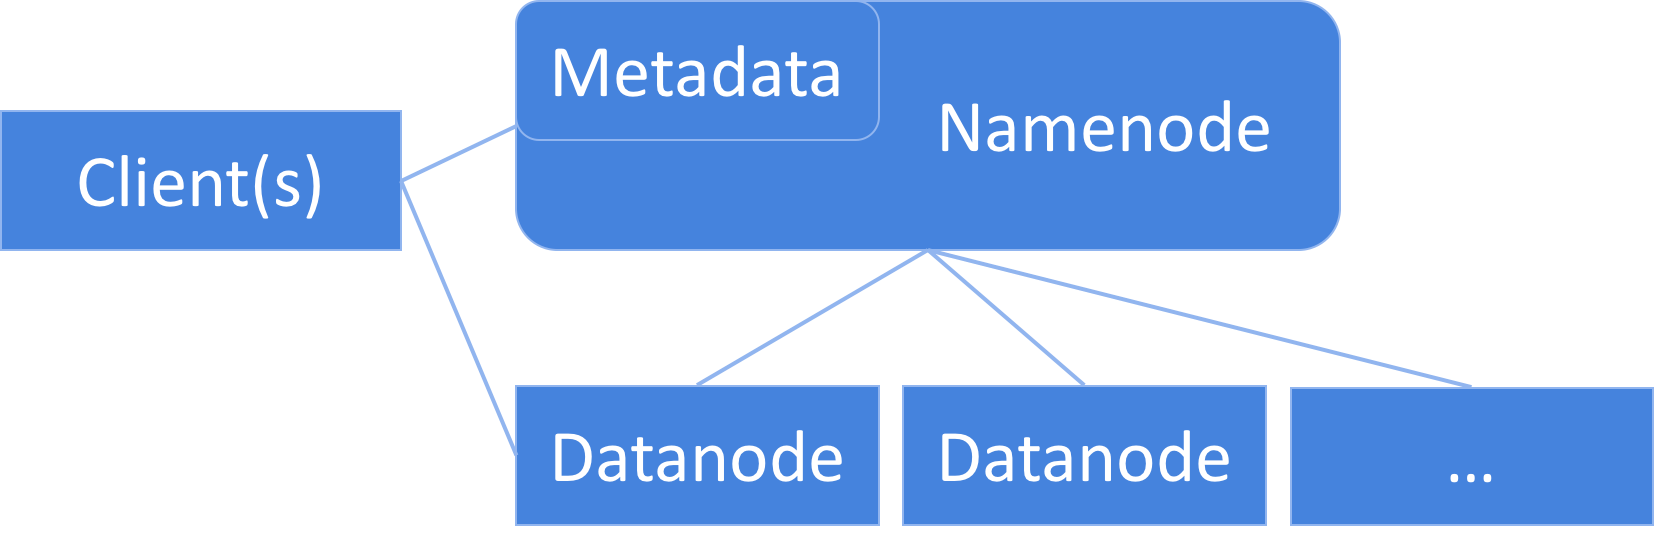
\includegraphics[width=1.0\textwidth]{images/hdfs-block-diagram.png}
\end{figure}

The HDFS system contains three main components, as shown in Figure \ref{fig:hdfs-block-diagram}:
\begin{enumerate}
\item one \emph{namenode}, with an optional hot standby copy,
\item a set of \emph{datanodes}, and
\item \emph{clients} interacting with the system.
\end{enumerate}

\paragraph{The namenode} is the central entity responsible for storing and applying modification to the system's metadata.
Metadata stored in the namenode includes information on the state and health of the cluster, information on how files are stored and replicated and finally information on the state of operations being executed.
Background threads in the namenode are also responsible for initiating periodic maintenance tasks such as block re-balancing and lease recovery.
It is a server application written in the Java programming language and it accepts commands from clients via the RPC interface mentioned above.
The namenode can also publish commands that will be executed by datanodes using the heartbeat mechanism.
The heartbeat mechanism is described in detail in Section \ref{sec:heartbeat}.
In HDFS the namenode is a single point of failure and, in the event of namenode failure, manual fail-over to a hot-standby is required to restore service availability.

\paragraph{Datanodes} are processes that handle physical storage of file blocks on disk.
A datanode is oblivious to the concept of file and only stores blocks.
To increase scalability, the datanode communicates directly with clients during read operations and with clients and other datanodes during write operations.
It also periodically reports its health and the integrity of the blocks it manages to the namenode via heartbeats.

\paragraph{Clients} are all programs that interact with the system to create, append or read files stored in the distributed file system.
As mentioned above, clients may be written in any language for which a protocol buffer implementation is available.
Depending on the operation type, client may interact with both namenode and datanodes to complete an operation.

While for some operations, such as listing the content of a directory, the client only performs a RPC call to the namenode, read and write operations require the client to contact both the namenode and datanodes.
HDFS follows a single-writer multiple-reader semantic for files, which means that there can be an arbitrarily large number of clients reading a file but only one writing data to it.

\subsubsection{Read pipeline}
When performing a read operation on a file, the client begins by contacting the namenode to get the addresses of the datanodes containing the first block of the file.
The list of datanodes holding a copy of the requested blocks is returned by the namenode sorted by proximity to the client requesting it according to the block placement policy.
The concept of proximity and how blocks are distributed onto datanodes is explained in Section \ref{sec:block-placement}.
The client then contacts the first datanodes to start reading the block.
If the connection to the datanode fails at any point during the operation, the client connects to the next datanode in the list and remembers the failed datanode so that it does not try to attempt a connection to it during following block reads.
If the checksum of the block read by the client is different from the expected one, the client communicates the checksum mismatch to the namenode before connecting to the next datanode in the list.
Once the client fully reads a block, it contacts the namenode to get the location of the next block and starts the process again.
In the actual implementation the client fetches several block locations with every call, further reducing the load on the namenode for client read operations.
It is worth mentioning that, on recent versions of Hadoop, the client can sometimes bypass the datanode completely and read the data directly from the local filesystem.
This operation is called a short-circuit local read.
The operation is only possible when the client is co-located on the same machine as the data-node housing the particular block requested, but this is often the case with data-aware frameworks such as MapReduce.

\subsubsection{Write pipeline}
\label{sec:write-pipeline}
Writes on HDFS are performed by one client at a time.
To maintain single-writer semantics, the client acquires a lease (essentially a lock) on every file it intends to write to.
The lease is periodically renewed by the client for as long as it is writing to the file.
If the lease is not renewed for a set amount of time, for instance because the client holding the lease crashed, it will expire.
There are two types of expiration times: soft, set at one minute and hard, set at 60 minutes.
When a lease expires after a soft timeout, it becomes available for other clients to claim through a procedure called \textit{lease recovery}.
On the other hand, when the hard limit for a lease expires, the namenode forcibly performs \textit{lease recovery} by closing the file, thereby making it available for new clients.
To decrease the network traffic generated by periodic lease renewal procedures on the namenode, a single lease renewal RPC call renews all the leases associated with the client performing the request.

Once the client acquires a lease, it contacts the namenode to get a new block id and a list of datanode to write data to.
The client will only write data and control messages such as \texttt{close}, to the first datanode which will then replicate the message to the second datanode in the list and so forth until there are no datanodes left.
Acknowledgments follow the same path in reverse, and are delivered in a single call to the client by the first datanode.
Finally, when the client closes the file, the lease is removed from the datanode and the block is closed by sending a close message through the pipeline.
The system is able to recover from failures during writing by performing \textit{pipeline recovery}.
Depending on the phase where the failure happens, the client can require a new set of datanodes from the namenode or exclude some of the datanodes from the pipeline.

\subsubsection{Block placement}
\label{sec:block-placement}
Apache HDFS stores a configurable number, three by default, of copies of each data block.
There are two primary reasons for this:
\begin{inparaenum}[i)]
\item to be able to withstand failure of a single data node holding the block and
\item to increase throughput by allowing different readers to read different copies of the same block
\end{inparaenum}.
To fulfill both purposes it is important to consider the placement of blocks in the context of the overall network topology where HDFS is deployed.
In a typical deployment, HDFS data nodes will be installed in server blades which will be installed in a rack.
Machines in a rack will be connected to the network via a TOR (top of the rack) switch, which will provide both connectivity between machines in the rack and connectivity to the other racks via a higher level switch. \footnote{insert image about network topology here} 
This type of deployment assumes that inter-rack connections are lower latency and have more bandwidth, while intra-rack connections are more expensive both in terms of bandwidth and latency.
In this scenario, each rack represents a separate failure domain, as failure of the TOR switch, loss of connectivity to the higher level switch, or power failure effectively isolates all the machines in the rack from the network.
To avoid the scenario where the loss of a single rack compromises the availability of all the replicas of a block, HDFS distributes the replica of a block across racks, provided that the cluster operator provides the namenode with information on placement of datanodes.

As part of the setup for a write pipeline, the namenode provides the client with a ordered list of datanodes to write data to.
If datanode rack placements are configured in the namenode, datanodes are selected as follows:
\begin{itemize}
\item If the client is in the cluster, like a MapReduce job, and there is a datanode on the machine, the first block is placed on the same machine as the client.
\item If, on the other hand, the client is not part of the cluster, the first block is placed on a random node as there is no way to compute a distance metric between the client and the datanodes.
\item The second block is placed on a machine in a different rack than the first block.
\item The third block is placed on another machine on the same rack as the second machine.
\item The fourth block, if present, is placed on a different machine on the same rack as the first machine.
\item If any more blocks are present, they are randomly distributed.
\end{itemize}
This distribution scheme minimizes the amount of inter-rack transfers necessary to spread the blocks on more than one availability zone.

\subsubsection{Fault tolerance}
Apache HDFS is designed as a modern distributed system and as such, datanode failure is treated as a routine event and handled transparently without the need for manual intervention.
Datanodes periodically communicate their health status to the namenode by sending heartbeat messages.
When a datanode stops sending heartbeat messages, the namenode considers it failed, and therefore it regards all the blocks stored on it as not accessible to the cluster.

To maintain the correct number of replicas for every block the namenode runs a background thread called the \textit{replication monitor}.
The replication monitor periodically checks the number of replicas for every block in the system and performs remedial action if the number is lower or higher than required.
\begin{itemize}
\item In case the block is \textbf{over-replicated}, the replication monitor schedules the deletion of the excess replicas in such a way that the remaining copies still fulfill the block placement policy.
\item In case the block is \textbf{under-replicated}, for example as a result of datanode failure, the replication monitor schedules the creation of new replicas according to the block placement policy.
\end{itemize}

The operations scheduled by the replication monitors are executed by datanodes and are transmitted to the relevant datanodes via the heartbeat mechanism.

\subsubsection{Heartbeat}
\label{sec:heartbeat}
The mechanism used by the datanodes to communicate their status to the namenode is to send periodic heartbeat RPC messages to the namenode.
The interval of time between heartbeats can be specified in the configuration file of HDFS but by default it is three seconds.
Responses to heartbeat messages from namenode to datanodes also optionally contain commands for datanodes to execute, such as the deletion of blocks, the re-replication of a block to another datanode, and so forth.
The main advantage of delivering commands as responses to heartbeats instead of sending commands from the namenode to the datanodes is that it allows a single namenode to manage a far greater number of datanodes, removing a bottleneck to scalability.

\subsection{Scalability limitations of HDFS}
\label{sec:scalability-limitations}
A study conducted regarding the scalability limitations of HDFS \cite{shvachko2010hdfs} concluded that HDFS can manage an estimate 1 petabyte of data per gigabyte of metadata.
While Apache HDFS can be scaled to manage multi-petabyte clusters, its single-active namenode design effectively limits both the amount of metadata and the number of queries per second (QPS) a node can process, to the largest machine it can be installed on.
The amount of metadata is limited because they are stored as Java objects in the Java Virtual Machine (JVM) heap space, which is itself limited by the amount of main memory available in the machine.
Furthermore, Java objects have a 8 to 12 byte header which is used by the virtual machine, increasing the memory requirements even further.
The amount of QPS that the system can process is limited by both the number and speed of processors in the machine, the connection between clients (including datanodes) and the namenode itself, and the number of alterations that the system can apply to the metadata.
Metadata objects are, in principal, only altered in two ways: from periodic processing by the namenode and as a consequence of RPCs invoked by clients and datanodes.
Given that any number of these alterations can happen in parallel, the namenode protects the metadata with a global lock, the \textit{FSNamesystemLock}, which can be acquired by an arbitrary number of threads in \emph{read} mode, but requires exclusivity when acquired in \emph{write} mode.
All operations that require modification of the metadata are therefore executed serially, further lowering the amount of queries per second that the namenode can process.
Storing metadata in the JVM heap is also problematic due to increasingly long garbage collection pauses that freeze the entire process as the heap grows in size.

\clearpage
\subsection{HopsFS}
\label{sec:hopsfs}
HopsFS \cite{DBLP:conf/fast/NiaziIHDGR17} is a fork of Apache HDFS created with the explicit goal of solving the biggest scalability and availability limits that are inherent to the single-namenode nature of the system: 
\begin{inparaenum}[i)]
    \item the amount of metadata limited by the main memory of the machine running the namenode process,
    \item the number and speed of processors in the machine,
    \item the amount and latency of bandwidth between the namenode and its clients,
    \item the coarse grained locking that requires a global lock to alter any piece of metadata, and
    \item the long garbage collection pauses can block the entire process for long periods of time as heap grows.
\end{inparaenum}
To do so, HopsFS decouples the responsibility of managing metadata from the namenode and places it in a separate distributed system called MySQL Cluster.
MySQL Cluster is a distributed, consistent (CP), in-memory relational database management system (RDMS) that can be operated and scaled independently from the hadoop cluster(s) it stores metadata for.
Data stored in MySQL Cluster's distributed storage engine (NDB), is divided between nodes participating in the cluster, allowing capacity to be increased by adding more machines to the cluster.
Unlike more traditional RDBMS, where data is stored on disk and only loaded in memory at query time, data in MySQL Cluster is stored in-memory and persisted to disk as a recovery mechanism, allowing very fast query execution.
By moving metadata to such a system, all of the issues regarding the memory limitations of a single system are automatically solved.
The gains are even more significant with regards to the amount of queries per seconds that the system can manage.
Decoupling metadata management from the namenode makes it a stateless component, which can be horizontally scaled and enables downtime-free failover, which is described in the following section.
Furthermore, compared with the approach of having a global lock for all metadata, a relational system \footnote{describe relational database, concept of row and lock on a row} such as MySQL Cluster can have much more fine grained locks allowing, for instance, parallel modification of the information of any number of different files.
Unlike memory-managed applications, MySQL Cluster also does not suffer from garbage collection pauses, avoiding the pitfall in performance as the amount of managed metadata grows larger.

\subsubsection{Multi-namenode architecture}
The namenode, which is now a client of the metadata storage system, performs metadata queries, both in terms of reading and modifying, using an interface called the (meta)Data Access Layer or DAL, which internally connects to the distributed storage system in an efficient fashion.
This allows multiple HopsFS namenodes to run in parallel, each serving a subset of the client requests to the overall system.
The architecture of the resulting system is shown in Figure \ref{fig:hopsfs-architecture}.

While most client operations can be directed to any one namenode, the block reports from datanodes and the daemon threads must be handled carefully.
In a Apache HDFS namenode, background daemon threads are responsible for a variety of functions including block re-balancing and lease recovery.
If allowed to run on every node in the cluster, these daemon threads would interfere with each other's work, causing unpredictable results.
To maintain the behaviour of Apache HDFS, HopsFS must guarantee that only one node in the cluster executes daemon threads at any given time.
To this end, all namenodes active in a cluster participate in a leader election algorithm, explained in detail in Section \ref{sec:leader-election}, that will elect a single namenode to be leader at any given time.
Additionally, the leader election procedure serves as \emph{failure detector} within the set of namenodes, allowing clients to retrieve a list of live nodes.
Datanodes fetch an updated list of active namenodes before every heartbeat messages, allowing them to keep an updated view of participants in the cluster and the current leader node's identity.
As metadata about the state of datanodes, the action they should execute, and the blocks they contain is stored in MySQL Cluster, any namenode can process heartbeats or block reports from any datanode.
Heartbeats are sent by the datanodes to different namenodes in a round-robin fashion, while the namenode to send block reports to is obtained by performing a RPC call to the leader.
The leader will assign the block report to a namenode that has the capacity to process it and has the lowest number of block reports to process at the moment where the RPC is sent.

\begin{figure}[h]
\caption{Architecture diagram of HopsFS. The metadata storage engine is provided by MySQL Cluster}
\label{fig:hopsfs-architecture}
\centering
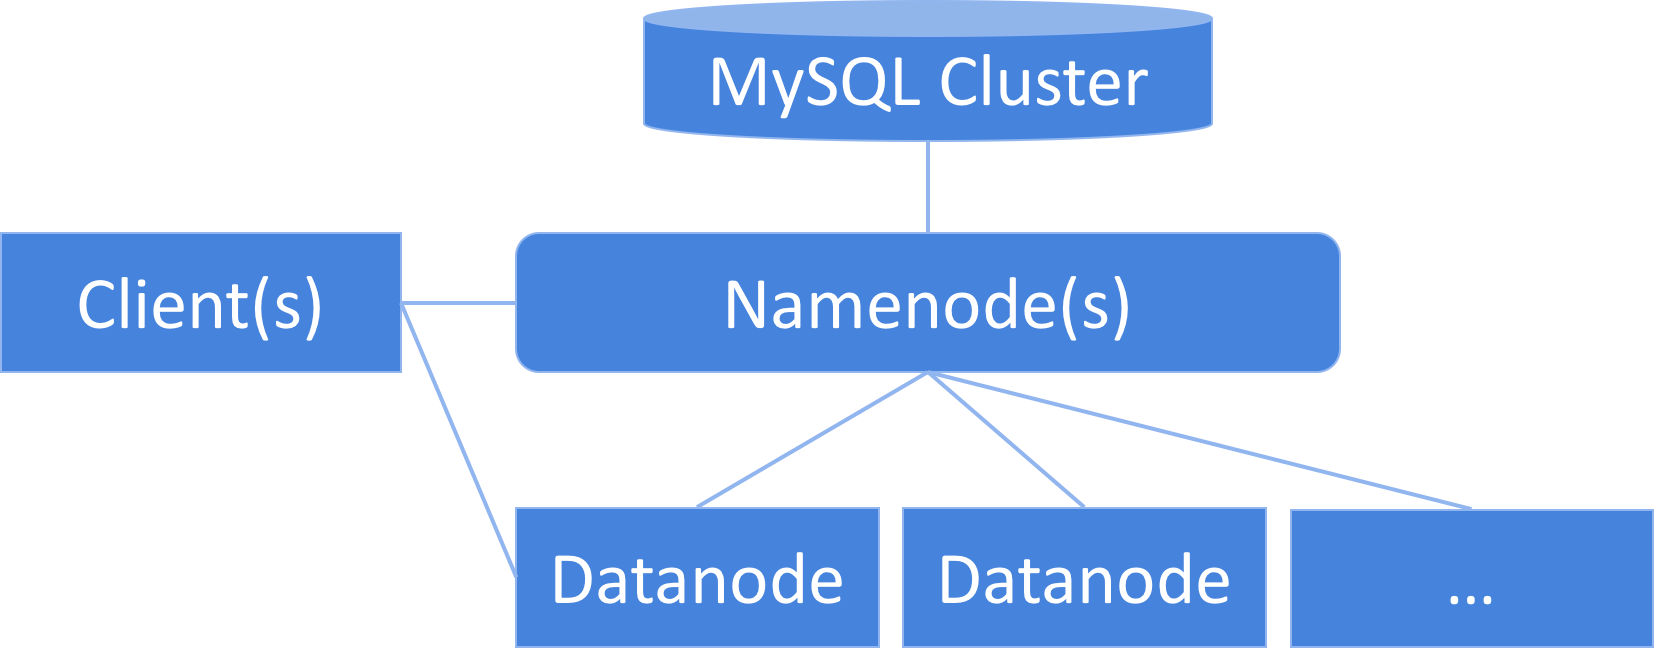
\includegraphics[width=0.9\textwidth]{images/hopsfs-block-diagram.png}
\end{figure}

\subsubsection{Group membership service and leader election}
\label{sec:leader-election}
As previously mentioned, HopsFS maintains a list of active namenodes in the system and elects one leader which executes functions critical to the proper functioning of the overall system.
Apache HDFS, when configured in High Availability mode (HA) also require such a system and leverages Zookeeper to perform these functions.
HopsFS eliminates the reliance on Zookeeper by leveraging the metadata storage system as shared memory and implementing reliable failure detection and leader election \cite{DBLP:conf/dais/NiaziIBD15} using MySQL Cluster distributed engine (NDB).
The failure detector implemented therefore complies with the requirements for the weakest failure detector for solving consensus  \cite{DBLP:journals/jacm/ChandraHT96}.

\subsubsection{The (meta)Data Access Layer}
\label{sec:dal}
The Data Access Layer, DAL for short, is the Hops component that allows the delegation of metadata handling to the MySQL Cluster database.
To achive this, the component provides two distinct pieces of functionality:
\begin{inparaenum}[i)]
    \item management of the life-cycle of database connection, including various optimizations to reduce network round trips and,
    \item abstractions that allow engineers working on Hops to convert all memory metadata accesses in database operations in a convenient way.
\end{inparaenum}
Formally, the data access layer provides only the interfaces that Hops itself uses to describe accesses to metadata, delegating the implementation of database access to a further library that provides concrete implementations.
Given that in Hops only one such implementation exists (\textit{hops-metadata-dal-impl-ndb}), this chapter will consider both DAL and DAL-implmenetation as a whole without making the distinction explicit.

\paragraph{Connection management}
The DAL provides management of the life-cycle of database connections to a MySQL Cluster cluster.
Specifically, upon configuration, the DAL creates two persistent connectors to the same MySQL Cluster cluster: one that connects to NDB using the native protocol and the ClusterJ java library and one that connects to SQL nodes using the standard JDBC MySQL driver.
The reason to use both a SQL driver and the native NDB protocol is that, while the NDB protocol is very fast at performing primary-key based operations, more complex operations such as joins and deletes are not supported and can only be executed through the SQL nodes.
Given that the performance of Hops is determined mostly by how fast it accesses metadata, the DAL must be as performant as possible.
To achieve better performance, this part of the DAL library implements optimizations aimed at reducing connection overhead, thus allowing a greater number of operations per second.
The main technique for this is connection pooling, which associates each open connection to a thread that will use it for all operations.
By allowing a thread to re-use the same connection for all operations, the overhead of opening the connection is effectively eliminated.
Connections are only closed in case of shutdown of Hops or errors on the connection itself, in which case the connection is re-opened at the next use. 
The connector itself is provided to clients as a global object, accessible to any component that requires it and it is initialized and configured in \texttt{Namenode.java}.

\paragraph{Database access}
Aside from managing database connections, the DAL provides abstractions that are used to convert all memory metadata accesses into accesses to the metadata storage layer.
The main abstraction provided is the \emph{request handler}, a structure that provides information on the type of operation being performed (the \texttt{OPCODE}) and the procedure to execute on the metadata, whether read-only or a modification.
When the handler is executed it performs the procedure in the context of a database transactions where errors will be handled by rolling-back the transaction itself, guaranteeing atomicity of metadata modifications.

The DAL provides two types of request handlers, the \emph{lightweight request handlers} which execute the operations as described above and the \emph{transactional request handlers} that apply most metadata modifications in memory before committing them to the database with the goal of reducing database round-trips.

In a \emph{lightweight request handler}, shown in Listing \ref{lst:lrh}, every modification to the metadata is concretely executed as a database query, causing a large number of network operations.
In case of transaction handlers with very large number of modifications, the network round-trips rapidly become the performance bottleneck.

To increase performance in modification heavy handlers, \emph{transactional request handlers}, shown in Listing \ref{lst:trh}, operate in a different way with the goal of reducing network operations to a minimum.
Transactional request handlers introduce a lock acquisition phase which is executed before the code for the transaction itself.
In this phase, the DAL acquires locks on all the specified rows and materializes them as objects in the DAL memory.
Upon execution, the handler operates on the in-memory representation of the objects either by modifying or deleting existing ones or by creating new ones through the \texttt{EntityManager} class.
At the end of the perform phase, the objects are divided into four categories:
\begin{inparaenum}[1)]
    \item unmodified,
    \item created,
    \item deleted,
    \item modified,
\end{inparaenum}
and the required operations are executed in batch on the database.
The perform phase is, therefore, still executed in the context of a database transaction, with the possibility of rollback in case of errors, but all operations on the database are executed at the end.
Given that all of the materialized rows are locked for the duration of the database, there can be no conflicts upon commit at the end of the handler.
Note that the handler can request read locks as well as write locks and, in that case, the rows locked in read mode cannot be modified.

Replacing all memory accesses with transaction handlers which acquire the minimum amount of locks required to perform the operation, HopsFS achieves a much more granular level of concurrency compared to the in-memory global lock, which allows it to execute a much greater number of concurrent operations.


\begin{lstlisting}[label={lst:trh}, caption={Transactional request handler for the rename operation}]
OperationType opType
if(isUsingSubTreeLocks) {
    opType = HDFSOperationType.SUBTREE_RENAME;
} else {
    opType = HDFSOperationType.RENAME;
}
new HopsTransactionalRequestHandler(opType, src) {
    @Override
    public void acquireLock(TransactionLocks locks)
    throws IOException {
        LockFactory lf = LockFactory.getInstance();
        locks.add(lf.getRenameINodeLock(
            nameNode, INodeLockType.WRITE_ON_TARGET_AND_PARENT,
            INodeResolveType.PATH, true, src, dst))
        .add(lf.getBlockLock())
        .add(lf.getBlockRelated(
            BLK.RE, BLK.CR, BLK.UC,
            BLK.UR, BLK.IV, BLK.PE, BLK.ER));
        if (dir.isQuotaEnabled()) {
            locks.add(lf.getQuotaUpdateLock(
                true, src, dst));
        }
        if (!isUsingSubTreeLocks) {
            locks.add(lf.getLeaseLock(
                LockType.WRITE))
            .add(lf.getLeasePathLock(
                LockType.READ_COMMITTED));
        } else {
            locks.add(lf.getLeaseLock(
                LockType.WRITE))
            .add(lf.getLeasePathLock(
                LockType.WRITE, src));
        }
        if (erasureCodingEnabled) {
            locks.add(lf.getEncodingStatusLock(
                LockType.WRITE, dst));
        }
    }

    @Override
    public Object performTask(StorageConnector connector)
    throws IOException {
        if (NameNode.stateChangeLog.isDebugEnabled()) {
            NameNode.stateChangeLog.debug(
                "DIR* NameSystem.renameTo: with options - " + src + " to " + dst);
        }

        if (isInSafeMode()) {
            throw new SafeModeException("Cannot rename " + src, safeMode);
        }
        if (!DFSUtil.isValidName(dst)) {
            throw new InvalidPathException("Invalid name: " + dst);
        }
        for (MetadataLogEntry logEntry: logEntries) {
            EntityManager.add(logEntry);
        }

        for (Options.Rename op: options) {
            if (op == Rename.KEEP_ENCODING_STATUS) {
                INode[] srcNodes = dir.getRootDir()
                    .getExistingPathINodes(src, false);
                INode[] dstNodes = dir.getRootDir()
                    .getExistingPathINodes(dst, false);
                INode srcNode = 
                    srcNodes[srcNodes.length - 1];
                INode dstNode = 
                    dstNodes[dstNodes.length - 1];
                EncodingStatus status = EntityManager.find(
                    EncodingStatus.Finder.ByInodeId, dstNode.getId());
                EncodingStatus newStatus = new EncodingStatus(status);
                newStatus.setInodeId(srcNode.getId());
                EntityManager.add(newStatus);
                EntityManager.remove(status);
                break;
            }
        }

        removeSubTreeLocksForRenameInternal(
            src, isUsingSubTreeLocks, subTreeLockDst);

        dir.renameTo(
            connector, src, dst, srcNsCount,
            srcDsCount, dstNsCount, dstDsCount, options);
        return null;
    }
}.handle(this);
\end{lstlisting}

\begin{lstlisting}[label={lst:lrh}, caption={Lightweight request handler }]
new LightWeightRequestHandler(UsersOperationsType.GET_USER_GROUPS) {
    @Override
    public Object performTask(StorageConnector connector)
    throws IOException {
        boolean transactionActive = connector.isTransactionActive();

        if (!transactionActive) {
            connector.beginTransaction();
        }

        Integer userId = cache.getUserId(userName);
        
        User user;
        if(userId == null) {
            user = userDataAccess.getUser(userName);
        } else {
            user = userDataAccess.getUser(userId);
        }

        if (user == null) {
            return null;
        }

        List<Group> groups = userGroupDataAccess
            .getGroupsForUser(user.getId());

        if (!transactionActive) {
            connector.commit();
        }

        return new Pair<User, List<Group>>(user, groups);
}.handle(this);
\end{lstlisting}
\subsection{MySQL Cluster}
\label{sec:mysql-cluster}
HopsFS delegates the storage and querying of metadata to an external database called MySQL Cluster.
MySQL Cluster is a in-memory, distributed, consistent, relational database management system (RDBMS) currently developed by Oracle.
The sources for the system are released under the terms of the GNU General Public License (GPL), but development is driven by Oracle without external contributors.
MySQL Cluster is the combination of the MySQL relational database management system and a distributed table storage system called Network DataBase (NDB).
As such, any program that is able to use MySQL as the database can be migrated on a MySQL Cluster system with minimal modifications.

\subsubsection{Network DataBase}
NDB is a in-memory share-nothing database which runs as a distributed application on a set of nodes.
Its share-nothing architecture relies on message passing between nodes participating in the cluster instead of disk or memory sharing like other distributed databases.
Furthermore, unlike traditional databases, NDB holds all data for tables in main memory.
Each NDB cluster contains two sets of nodes: \begin{inparaenum}[i)]
    \item data nodes, \texttt{ndbd} and \texttt{ndbmtd}, which contain the data for tables and participate in queries and commit protocols
    \item management nodes, \texttt{ndbmgmt}, which provide parameters to data nodes in order to form and maintain clusters and, typically, act as \emph{arbitrators} during split brain protocol 
\end{inparaenum}.
In NDB tables are divided into \emph{partitions} and partitions are assigned to node groups.
In order to compute the partition any row belongs to, the default strategy is to take the hash of the primary key modulo the number of node groups, tough this behaviour can be modified at table creation time.
The system can be configured, by tuning parameters in the management node(s), to replicate each data partition multiple times.
Aside from creating redundancy in case of data node failure, multiple data nodes will be able to serve reads for the partitions stored in the node group, linearly increasing the number of read queries per second that the system can serve.
If replication is set to one, only one copy of the data is available in the system and, if the data node storing the partition fails, the data is permanently lost.
If replication is set to a value higher than one the cluster is divided in logical units called node groups.
The number of node groups $N_g$ formed is controlled by $N_g = \frac{N_t}{R}$ where $N_t$ is the total number of data nodes in the system and $R$ is the replica factor.
This also implies that, by setting the replica factor $R$, the number of datanodes in the cluster must necessarily be a multiple of $R$ itself.
Every write for a data partition will be replicated on every node in the assigned replica group so that, in case of failure of any node, the system will still be able to serve all the requests, albeit at a slower rate.
Image \ref{fig:ndb-node-groups} shows an example scenario for a cluster with $N_t = 12$ and $R = 3$.

\begin{figure}[h]
\caption{Node groups}
\label{fig:ndb-node-groups}
\centering
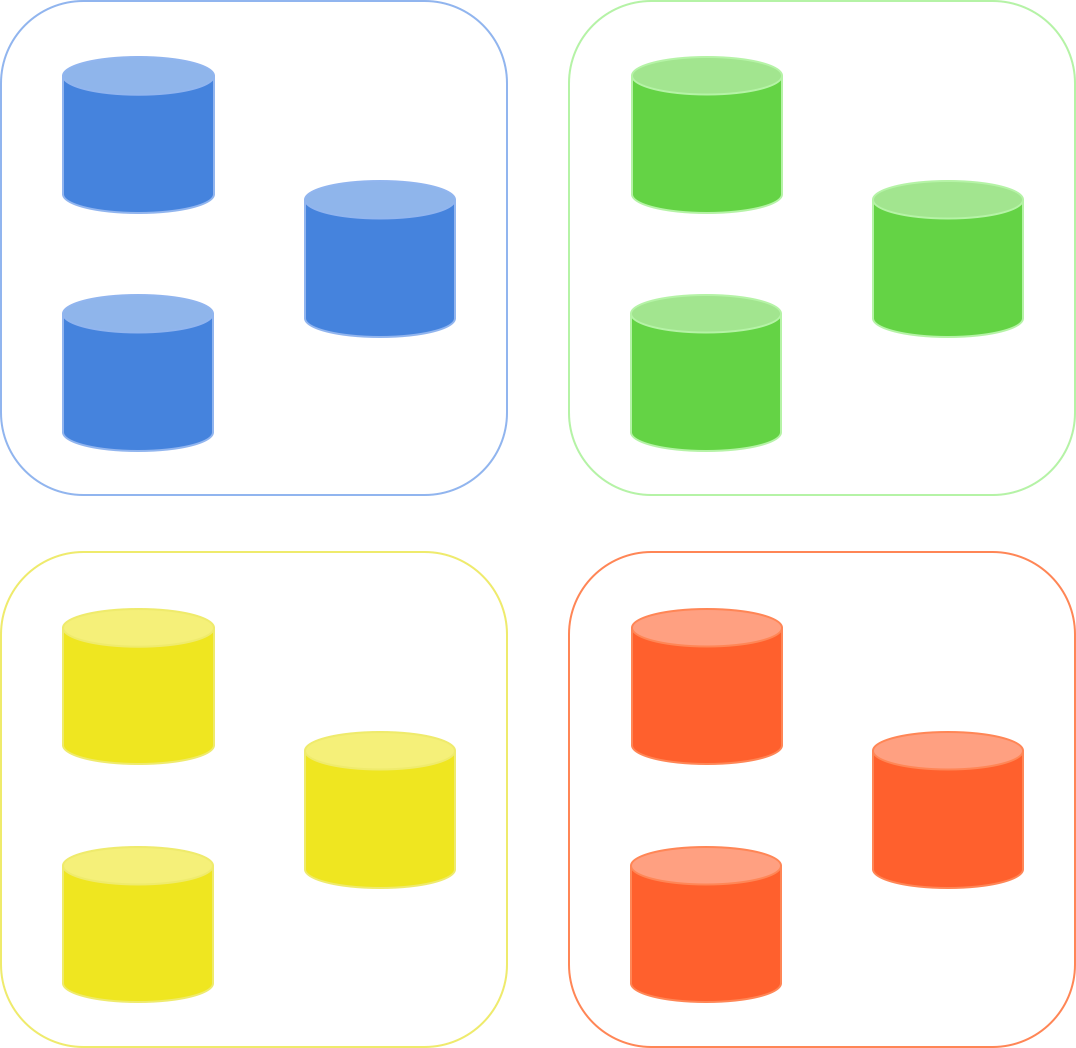
\includegraphics[width=0.95\textwidth]{images/ndb-node-groups.png}
\end{figure}

In order to provide clients with synchronous transaction, which maintain data consistency, NDB employes a two phase commit protocol (2PC) \cite{bernstein1987rrency} when committing transactions.
A 2PC protocol run is divided into two phases: \begin{inparaenum}
    \item a \emph{prepare} phase, where nodes execute the operations specified in the transaction and prepare for a commit
    \item a \emph{commit} phase, where nodes commit the operation
\end{inparaenum}.
After a successful \emph{commit} phase, the data is durable and cannot be rolled back by any node.
To initiate a transaction, a client contacts any data node.
Data nodes contain a \emph{transaction coordinator} process, which identifies the partitions involved in the transaction and initiates the 2PC protocol.
If any node involved in the transaction fails, the transaction coordinator will abort the transaction after a short timeout of 5 seconds by default.
Clients of the system are expected to handle transaction failure, and the typical strategy is for the client to retry the transaction at a later time.

To detect failures, data nodes arrange themselves in a virtual ring and send heartbeat messages to the next node in the circle.
If one node fails to acknowledge a heartbeat three consecutive times, it is considered failed and the cluster enters a split brain protocol, during which it is not able to accomplish any work.
The purpose of a split brain protocol is to identify and designate a subset of nodes in the cluster that still have a complete copy of all partitions and can therefore continue to function, albeit in a degraded fashion.
To identify the \emph{sub-cluster} that continues to function, each sub-cluster executes a series of checks:
\begin{itemize}
    \item if the sub-cluster includes all nodes from any node group, this is the only possible functional sub-cluster and can \textbf{continue to operate},
    \item if the sub-cluster does not contain at least one node in each node group, this sub-cluster is not functional and can \textbf{shut-down},
    \item if the above conditions are both false, there is more than one functional sub-cluster, \textbf{defer the decision to an arbitrator}.
\end{itemize}
In order to avoid a split brain scenario, where two or more subsets of the cluster continue to apply diverging modifications to the data in parallel, the arbitrator allows only one of the functioning clusters to continue.
The arbitrator select only one cluster by only replying positively to the first subset contacting it, instructing all following sub-clusters to shutdown.
If a sub-cluster cannot contact the arbitrator within a predefined amount of time, it shuts itself down, guaranteeing that \emph{at most} one sub-cluster will be live during split brain protocol.
The role of arbitrator can be fulfilled by both management nodes and SQL nodes, which are explained below, but management nodes have higher priority compared to SQL nodes.
Given that, without an arbitrator the whole cluster fails upon failure of a single node, more than one node can fulfill the role of arbitrator, albeit not at the same time.
If an arbitrator fails during normal cluster operations, the datanodes agree on another, selected from a list of arbitrators and associated priorities.
This list is specified at cluster configuration time and can only be updated by a management node by applying a configuration change.
All the nodes that shut down as part of the split brain protocol must re-join the cluster through a management node upon restarting.
It is worthy to note that, while the cluster is effectively able to access all data in the aftermath of a split brain protocol, the reduced capacity of one or more node groups can cause load spikes for the nodes that are left.

NDB data nodes store all partition data in main memory.
In case of data node shutdown, either planned or unplanned, all the partitions on the node are lost.
While a restore procedure can, in principal, fetch copies of the partitions from other data nodes in the same node group this will either \begin{inparaenum}[1)]
    \item take a very long time if the goal is to minimize the impact on the other working nodes in the node group
    \item consume most of the bandwidth on the working nodes left in the node group, further worsening the strain caused by a reduced number of nodes in the group
\end{inparaenum}.
To limit the amount of bandwidth required by a node restore procedure, data nodes periodically checkpoint state to durable storage.
Checkpoints to durable storage are achieved by periodically flushing to disk a log, called the \emph{REDO} log, which contains all the transactions committed between the last flush and now.
To obtain a consistent snapshot of the system, one where no committed transactions have a dependency on uncommitted transactions, all the data nodes coordinate using a global checkpoint protocol (GCP).
GCP enables data nodes to flush REDO logs in such a way that the resulting snapshot is globally consistent.
Due to the way the REDO log stores changes, without any other mechanisms to limit its growth, the on-disk snapshot would effectively grow without bounds.
To prevent this, data nodes also run a local checkpoint (LCP), which persists a snapshot of the state of the partitions in the system to durable storage.
With a complete snapshot available, the node can discard the portion of REDO log coming before the local snapshot, as in case of restore the local state is used to reconstruct the in-memory state of partitions.
In case of restore a data node \begin{inparaenum}[i)]
    \item loads the most recent local checkpoint
    \item applies all the transactions from the REDO logs
    \item requests the newest transactions from other nodes in the group
\end{inparaenum}.
By using a combination of LCP and REDO log, the node therefore reduces the amount of data to transfer from a complete snapshot to only some transactions.
The above techniques only help if the node starts the restore relatively promptly as the local snapshots will be quickly invalidated when other nodes erase theis REDO logs to create a newer LCP.

\subsubsection{SQL Nodes}
SQL nodes are MySQL server instances that can create and interact with tables using the \texttt{NDBCLUSTER} engine.
Tables created with such an engine are stored on a NDB cluster.
SQL nodes participate in the cluster as clients and can also be elected arbitrators, tough usually with lower priority compared to management nodes.
Any number of SQL nodes can be connected to the same NDB cluster to better distribute the load and increase the availability of the service for MySQL clients.
While MySQL server itself is modified to connect and participate in an NDB cluster, clients can connect using standard MySQL client libraries, which allows unmodified applications to take advantage of the scalability and performance benefits of MySQL Cluster.

\subsubsection{Isolation levels and locking}
NDB only supports transaction isolation level \texttt{READ\_COMMITTED}, which guarantees that uncommitted values will never be read.
While reading an uncommitted value is impossible, NDB implements READ COMMITTED on a row-by-row basis, which makes it entirely possible for a transaction to commit some updated values while another transaction is reading them, resulting in the second transaction observing a subset of values before the transaction and the rest after.
In concrete terms, whenever a data node receives a read request, it will always return the most recently committed value.

In order to obtain stricter forms of serialization, NDB allows transactions to set row-level locks, both shared and exclusive, which are released upon transaction commit or roll-back.
Row level locking is the fundamental mechanic that allows HopsFS to provide consistent filesystem operations to clients as well as enable the use of NDB as shared memory for the leader election processes.

\subsubsection{Geographic clusters}
While a single NDB cluster offers strong consistency and good performance in the context of a data-center network, MySQL cluster also offers a variety of options to extend a cluster to more than one data-center.

The obvious solution to the problem of geographic clusters would be to set up data nodes in all locations and join them in a single cluster the same way it would be done in a single data-center.
This is not, however, a viable solution in most scenarios due to both assumptions in NDB and in the way data-center networks are designed.
NDB assumes all data nodes are running in a interconnected network where the latency and bandwidth to contact any other node in the cluster is generally constant, and it leverages this assumption to provide on-line transaction processing typical of a online transaction processing system (OLTP).
Timeouts for transactions are very short (5 seconds by default) and the failure detection mechanic is also sensitive to increased latency as it may confuse a latency spike with node failure.
A multi-data center network, on the other hand, would have very low latency and high bandwidth between nodes in the same data-center but comparatively higher latency and lower bandwidth between nodes in different locations.
Furthermore, connections between nodes in different locations would all share very few channels, while internal data-center networks tend to be very well connected.

The better alternative for geographical replication in MySQL Cluster is to use asynchronous replication features built into MySQL.
Asynchronous replication techniques are used in standard SQL databases such as MySQL and PostgreSQL to achieve a variety of functions such as performing analytics without compromising the database running online processing or creating standby replicas, ready to be promoted should the master fail.
In asynchronous replication a node referred to as master publishes a log-like stream of operations it executed, in the order they were executed.
A set of other nodes, referred to as slaves or followers, consume the log of operations and apply the same operation to the local representation of the data.
The state of followers is therefore consistent with the state of the master at some point in the past, even in case of master failure.
This technique is asynchronous because the master does not wait for followers before reporting success to the client, thus maintaining the low latency operational characteristic of a online database.
High latency only affects this process in that the state of followers on high-latency links will lag further behind the master's state.
In the MySQL Cluster system, asynchronous replication and the conflict detection and resolution functions associated, which are illustrated later, are delegated to SQL nodes which propagate events to other SQL nodes and apply the necessary changes to the tables in NDB.
This technique is used to implement many different systems, depending on the application's requirements.

\paragraph{Master-follower}
A very common technique used to implement replication in systems where write traffic is mostly constant but read traffic is variable, is to have a simple single master/multiple follower system (shown in Figure \ref{fig:master-follower}), where write traffic is only directed to the master and read traffic can go to any of the available followers.
Such a system offers eventual consistency semantics for reads as followers may serve an outdated view of the master's state.
If a stronger consistency level is required, for instance by a client which needs a read-your-writes level of consistency, the only solution is to perform such reads on the master node.
While this system is relatively simple to implement and operate it is unsuitable for systems where write traffic (or consistent read traffic) increases to the point where it can no longer be handled by a single master.

\begin{figure}[h]
\caption{Master-follower topology}
\label{fig:master-follower}
\centering
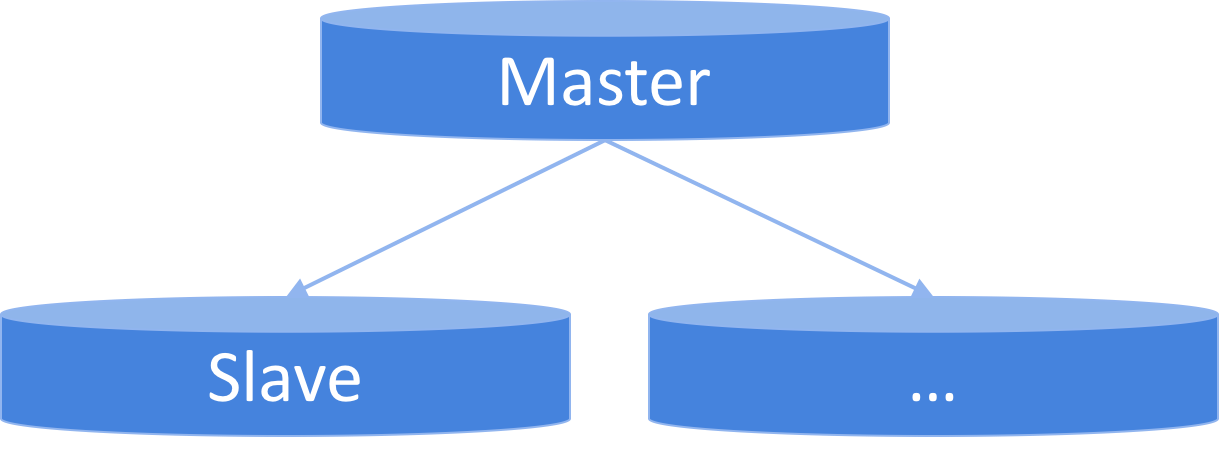
\includegraphics[width=0.95\textwidth]{images/master-slave.png}
\end{figure}


\paragraph{Balanced master-follower}
A solution which allows better scaling of write traffic is the so called Balanced master-follower or Partitioned Active/Active scheme.
In this scenario all of the nodes are configured as master for some partition of the data, while they act as followers for all other partitions, as shown in Figure \ref{fig:balanced-master-follower}.
Given that master or follower in this case is ambiguous we refer to nodes as either active or passive for a given partition.
Data partitioning can be done at the database, table or even row level, depending on the application.
The application is also responsible for selecting a partitioning scheme that distributes load evenly on all partitions.
Aside from increased complexity in the application, the system also requires a sophisticated routing system which guarantees that write operations always access the correct node which is active for the partition.
Fail over also requires care as one of the nodes may become overloaded if it becomes active for too many partitions.
While this system improves on the write scalability limits posed by the master-follower design, it still requires complex routing to perform writes.
The routing is necessary so that, when two applications try to write conflicting data, the writes are effectively serialized at the active partition, which will reject one of the two writes thus implementing consistent writes.

\begin{figure}[h]
\caption{Balanced master-follower topology}
\label{fig:balanced-master-follower}
\centering
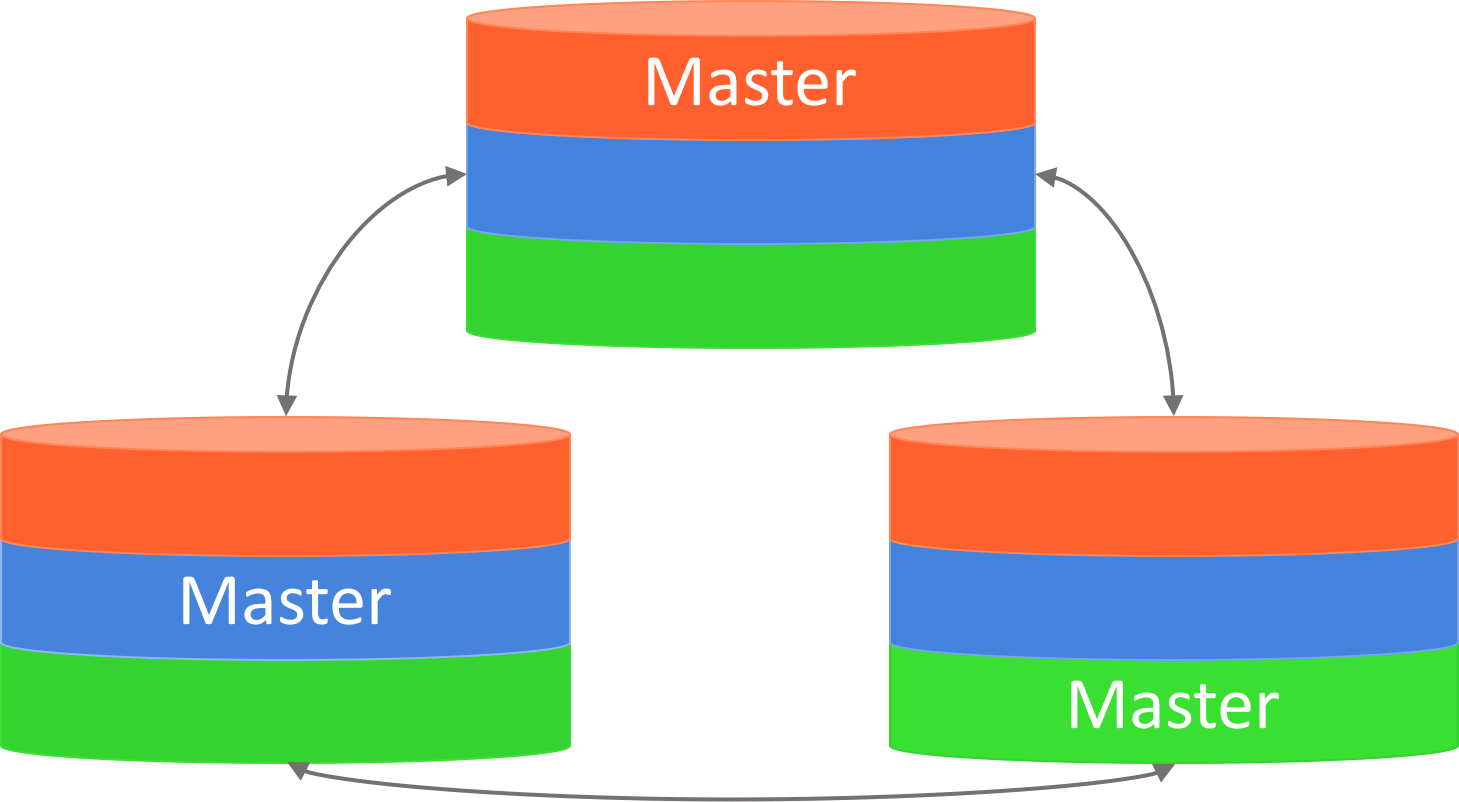
\includegraphics[width=0.95\textwidth]{images/balanced-master-follower.png}
\end{figure}

\paragraph{Optimistic Active Active}
In many parallel applications, conflicting operations are relatively rare, when compared to the total volume of write traffic.
While pessimistic systems such as master-follower or balanced master-follower simply make it impossible for write conflicts to happen, at the expense of limited write scalability or more complex routing logic, optimistic systems handle conflicts as they arise.
The core principal behind this assumption is that, while handling conflicts may be expensive, it is a very rare operation and the total cost is therefore inferior to the constant cost of serializing writes in a master/active node.
An optimistic active active replication system, shown in Figure \ref{fig:optimistic-active-active}, allows write traffic on any node part of the cluster.
When a transaction is committed, it is propagated asynchronously to the other nodes which will check for conflicts. If a conflict is detected it is rolled back.
Clients of such a system must accept that they may read data which is stale or not durable because it may be rolled back, but the overall system is much more scalable and does not require complex routing as both reads and writes can be executed at any node.

\begin{figure}[h]
\caption{A topology with two MySQL Cluster clusters replicating with active to active configuration}
\label{fig:optimistic-active-active}
\centering
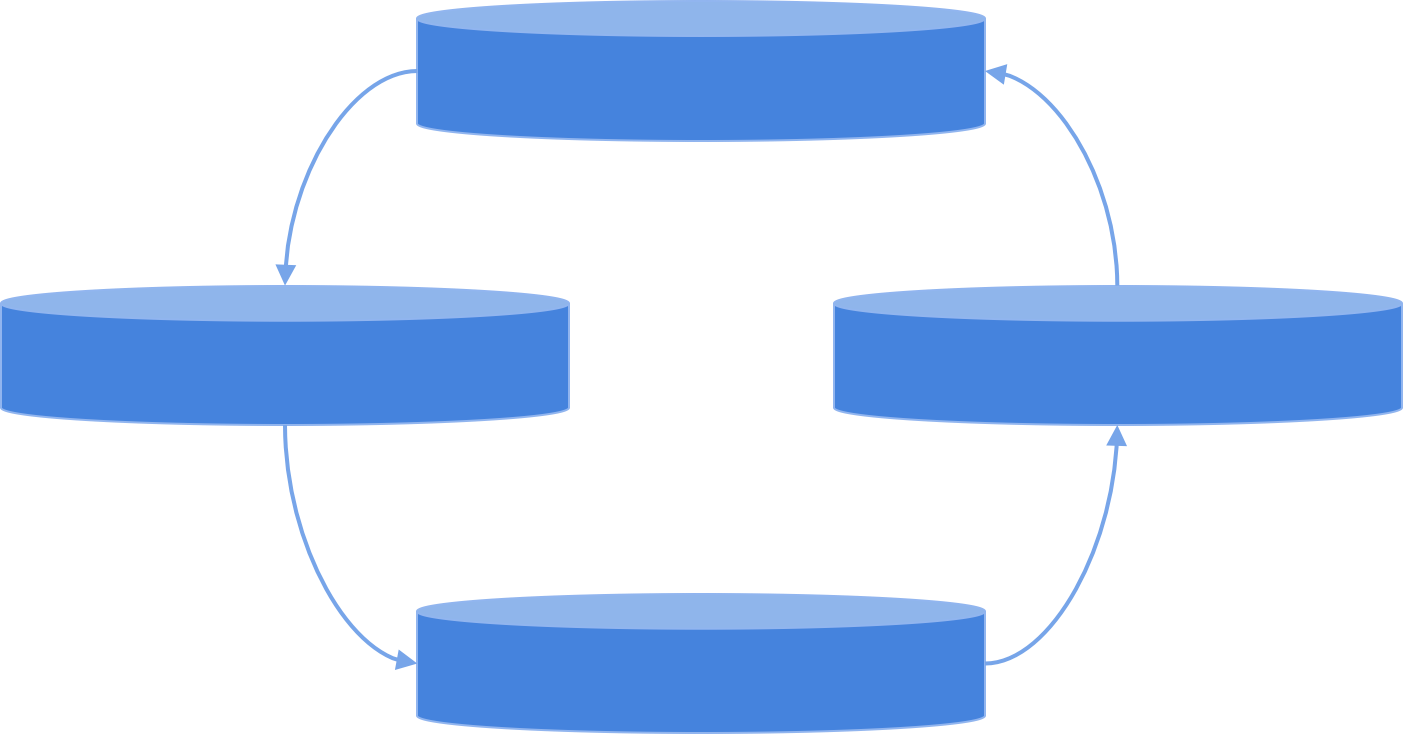
\includegraphics[width=0.95\textwidth]{images/optimistic-active-active.png}
\end{figure}

\paragraph{Hybrid Optimistic Active Active}
A hybrid optimistic active active system, shown in Figure \ref{fig:hybrid-optimistic-active-active} works like its purely optimistic counterpart with the additional advantage of defining an active node for each partition.
Writes performed on the active node for the partition will be durable and will not be rolled back, while writes on other nodes will be rolled back if they are in conflict with those originating on the active node.
This system still enables the benefits of the optimistic active active scheme, by routing traffic to the passive nodes while allowing applications that require write consistency or read-your-write semantics to be routed to the active node for the partition.

\begin{figure}[h]
\caption{Hybrid optimistic active to active topology}
\label{fig:hybrid-optimistic-active-active}
\centering
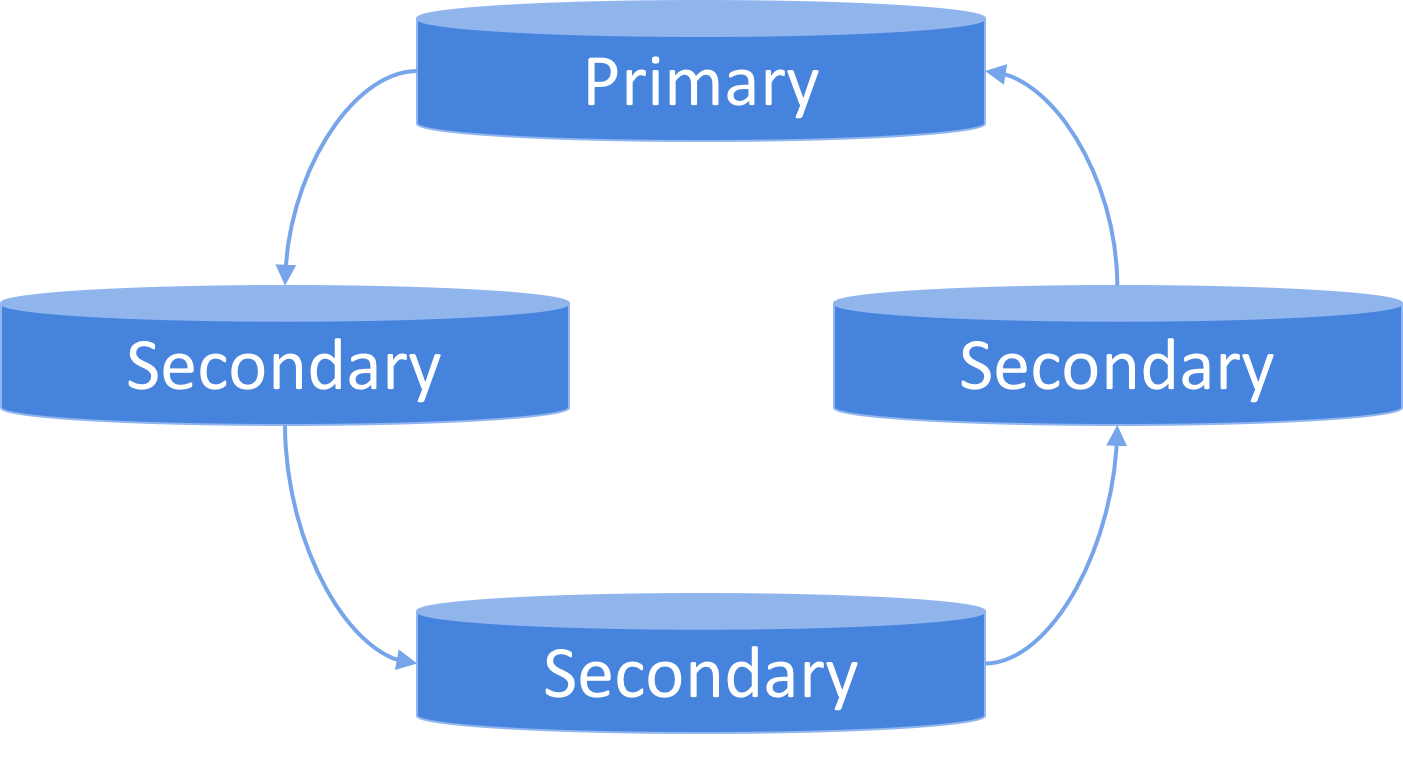
\includegraphics[width=0.95\textwidth]{images/hybrid-optimistic-active-active.png}
\end{figure}


\subsubsection{Dealing with conflicts in optimistic configurations}
Optimistic systems require the ability to detect conflicting updates and reject them in order to avoid diverging replica states.
Rejection is not, however, the only strategy to avoid diverging replica states, as many conflict can instead be merged by the application depending on specific application logic.
In the simple case of a numeric value which is set to 1 and is incremented by 1 on each replica, rejecting one of the updates would result in a value of $2$ but an application could merge the conflicting updates, producing a correct value of 3.

MySQL Cluster provides a sophisticated mechanism to both detect and resolve (merge) conflicts in a optimistic active active replication scheme.
All of the available methods are documented in the MySQL Cluster documentation website \cite{mysql-cluster-documentation-replication}, but this section gives an overview of the \texttt{NDB\$EPOCH} and \texttt{NDB\$EPOCH\_TRANS} merging functions, which can detect and resolve conflicts at a transaction granularity.
The \texttt{NDB\$EPOCH} functions can only be applied in the context of a hybrid optimistic active active system with two replicating clusters as shown in Figure \ref{fig:two-active-active-clusters}.
Partitioning of data in this case can be either at table or database level, but this chapter will assume only one database configured as active on one cluster and passive on the other.
We will refer to the active cluster as \emph{primary} and to the passive cluster as \emph{secondary}.
As previously mentioned, the hybrid optimistic setup implies that all writes performed on the primary cluster are durable, while all writes on the secondary cluster may be rolled back.
As shown in Figure \ref{fig:two-active-active-clusters}, one SQL node per cluster acts as both master publishing changes for the other cluster to consume and follower fetching changes from the other cluster, tough this is not the only possible set-up.
The resulting setup is a circular replication scheme, which is necessary for the conflict detection and merging functions to work.

\begin{figure}[h]
\caption{A topology with two MySQL Cluster clusters replicating with active to active configuration}
\label{fig:two-active-active-clusters}
\centering
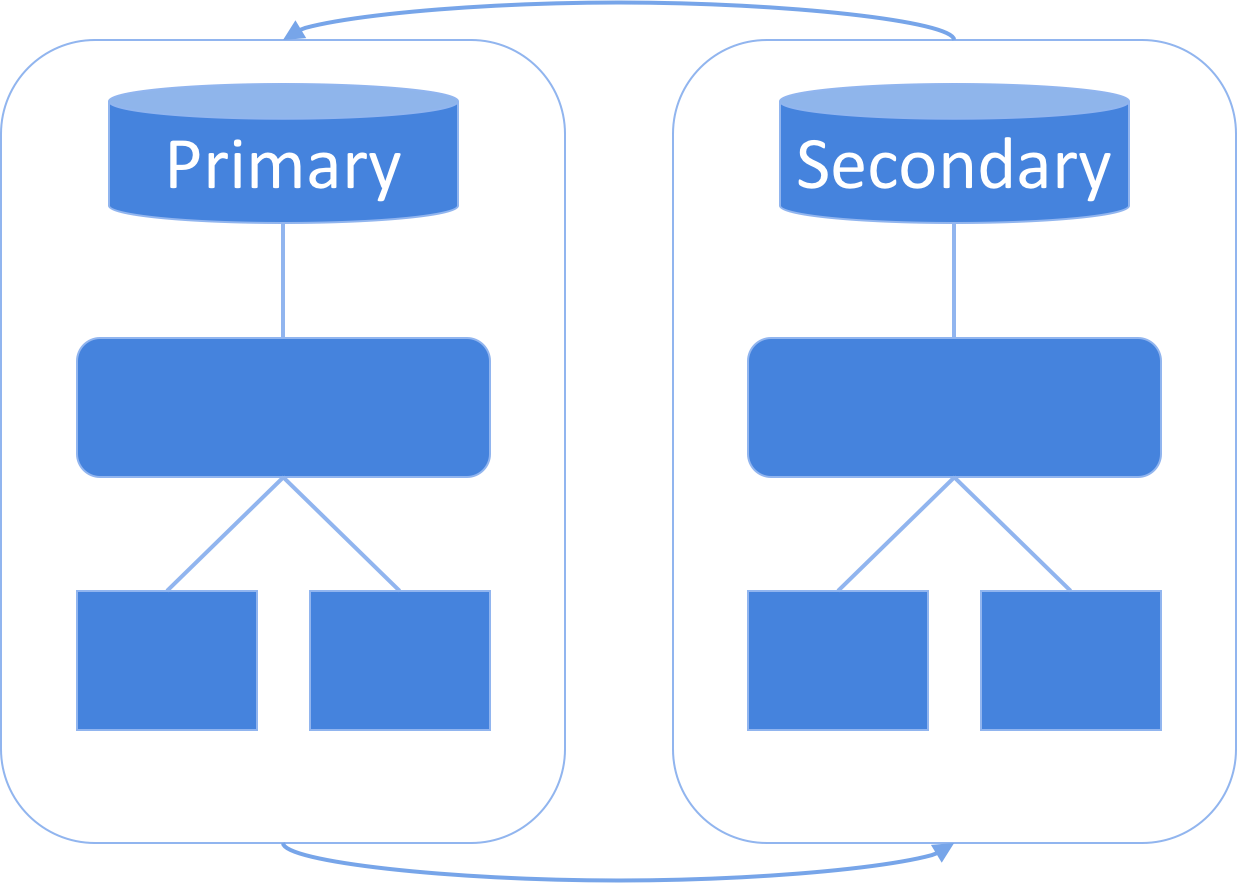
\includegraphics[width=0.95\textwidth]{images/hops-active-active.png}
\end{figure}


Conflict detection is performed on the primary cluster, as any conflicts caused by the primary cluster, which would be handled by the secondary cluster, are automatically ``won'' by the primary cluster.
When a conflict is detected the master emits events that re-align the secondary cluster with the state of the primary cluster, in effect rolling back any conflicting changes.
Here \texttt{NDB\$EPOCH} and \texttt{NDB\$EPOCH\_TRANS} diverge in behaviour: while the former only re-aligns the rows causing a conflict, the latter rolls-back the entire transaction and any transactions that depend on it before applying the master state.
Aside from aligning the secondary state to that of the primary, MySQL Cluster also provide a powerful mechanism for applications to merge conflicting state: the \emph{exception tables}.
Exception tables are created on the primary cluster with the same name as the tables conflict resolution is enabled for but with the additional \texttt{\$EX} suffix.
These tables include a variety of columns including all of the columns of the primary key for the original table, some columns containing information on the conflict itself, and optionally any other column from the conflicting table as well as meta-columns containing values before and after the exception itself.
If such tables are present when conflict resolution is enabled, every time a conflict is detected and the secondary state is re-aligned, the value for the aligned rows in the secondary is saved in the exception tables.
The application can then poll the exception tables to implement any desired merging behaviour.
Going back to the example of two concurrent transactions adding one to a value in a row, an entry for the secondary would be added in the exception table and the application would then be able to increment the counter again and delete the row from the conflict table to merge the results and obtain the correct value.

Finally, it is important to note that conflict detection is sensitive to replication latency between the two clusters and the longer replication latency is, the more likely it is for the clusters to produce conflicting transactions.

\subsection{HopsFS Database Optimizations}
\subsubsection{Metadata Partitioning}
\subsubsection{Hotspots}
\clearpage

\section{Literature review}
\label{sec:similar-systems}
This chapter analyzes the prior art in the space of distributed file-systems with a particular focus on the handling of metadata.
Given that Apache HDFS has already been described in detail, it is omitted from this section and three others are described instead.


\subsection{The Google File System}
The Google File System (GFS) \cite{DBLP:conf/sosp/GhemawatGL03} is the distributed file-system employed internally by Google until it was replaced by Colossus, another internal system (which remains unpublished at the time of this writing). 
The design of GFS and MapReduce \cite{DBLP:journals/cacm/DeanG08} directly drove the implementation of the Hadoop platform and, as such, there are many similarities between GFS and HDFS.

\subsubsection{Architecture}
\begin{figure}[h]
\caption{GFS architecture diagram}
\label{fig:hdfs-block-diagram}
\centering
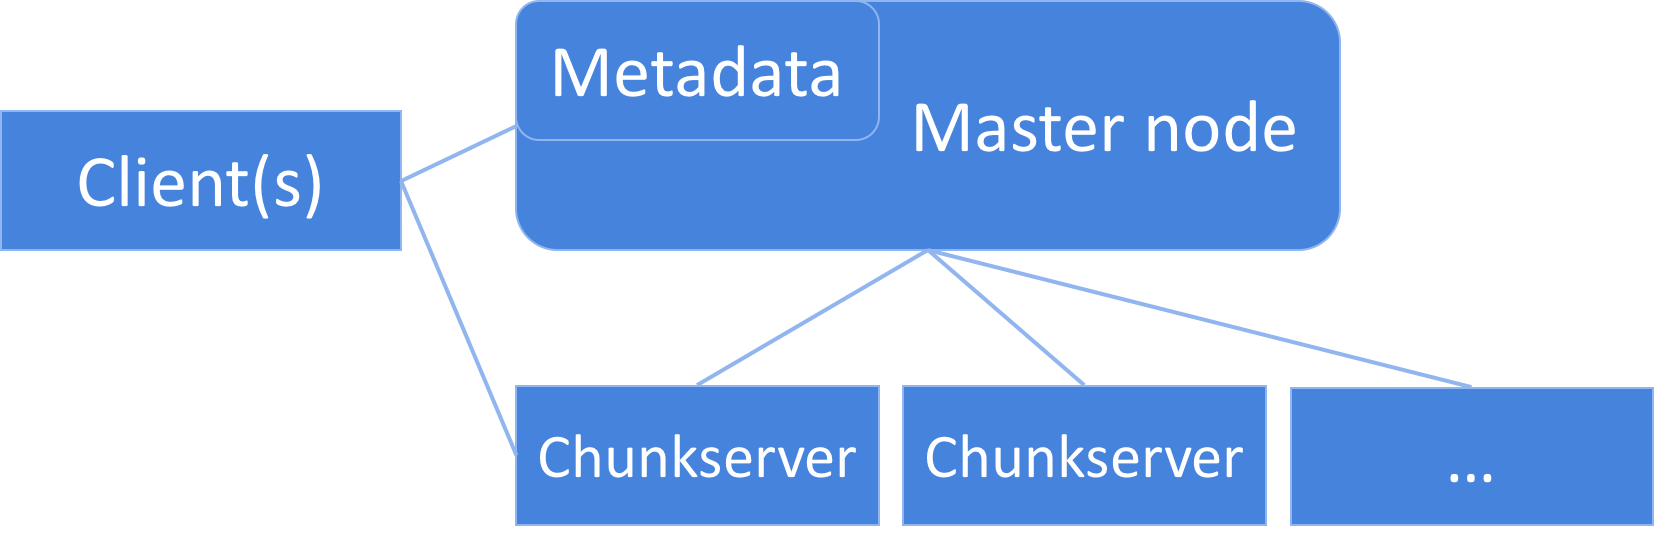
\includegraphics[width=1.0\textwidth]{images/gfs-block-diagram.png}
\end{figure}

GFS is designed as a distributed non-POSIX-compliant file-system for distributed applications and it is built by clustering a set of general-purpose machines as shown in Figure \ref{fig:gfs-architecture}.
It is a distributed system with three distinct roles: 
\begin{itemize}
    \item a \emph{master node}, which maintains metadata on files and the state of the system,
    \item a set of \emph{chunkservers} which perform storage of data on disk and directly interact with clients, and
    \item clients which read and write data from/to the system.
\end{itemize}
In the system files are divided in chunks, which can grow up to 64 megabytes before another chunk is created.
The master stores both the hierarchy of files and directories, as well as information on which chunks form any given file.
Multiple copies of each chunk (three by default), referred to as replicas, are managed by different chunckservers operating in different failure domains.
Chunks are stored as regular files in the chunkserver's local filesystem.
Replication is employed to maintain data availability in the face of chunckserver failure, as well as to provide a limited form of load balancing by allowing different clients to read different replicas of the same block.
The location of replicas is stored, alongside all other file metadata, in the master main memory.

As in HDFS, the single master node is the main scalability and reliability bottleneck for the system and, as such, many techniques employed in GFS have to goal of reducing interactions with this node to a minimum and increase its reliability.
\paragraph{Reads} The chunk size is purposefully very large compared to local file-systems, as any read request must first contact the master to learn the location of block replicas.
When responding to such a query, the master sends location data about several following blocks in the file and this information is cached by clients for a short period of time, to avoid excessive master involvement in sequential read scenarios.
After learning the location of blocks, the client can complete the read operation with no further involvement from the master node, by contacting the relevant chunkservers directly.
\paragraph{Writes} In order to minimize the master's involvement in write operation, the systems grants block leases to chunckservers.
When a client requests to mutate a block, either by writing or appending to it, the master selects three (assuming a default replication factor) chunkservers to receive the mutation: a \emph{primary} and two replicas.
The primary is granted a new lease to alter a block with data received by the client for as long as the lease is valid, unless it was already holding a lease for the specified block.
The chunckserver can periodically renew the lease by contacting the master node if it is still receiving data from clients.
At this point, the client pushes the data to all the chunkservers and waits for a confirmation that all of the replicas received the data.
When a confirmation is received the client contacts the primary and requires a write operation.
The primary serializes all writes (there may have been concurrent writes) and then applies them to the file stored on the local disk.
After it applied the state to the local file it contacts the replicas and asks them to write the changes in the same order.
Once it receives confirmation from all replicas, the write is finally acknowledged to the client.
\paragraph{Reliability} In order to increase the master reliability, all metadata mutations are persisted on a disk-based log which is both kept on the local machine and replicated to a number of others.
Client operations that involve metadata modifications are not acknowledged before this flush is completed.
Given that such a mutation log would grow without bounds, it is periodically compacted into a snapshot.
The snapshot is created by serializing the current master metadata on disk in a format that can be directly used to restore a master without any parsing.
When a master needs to recover from a crash, first it loads the most recent snapshot, then it applies all the modifications in the log before accepting any client queries.
This mutation log is also used to keep several ``shadow masters'' up-to-date with the state of the master.
Shadow masters cannot perform any metadata mutation but they can serve read requests, even in the event of master failure.
This mechanism is used both to scale the system further by delegating reads to a shadow master and to grant a read-only service during recovery of the master.

\subsubsection{Chunk management}
While client-initiated operations are optimized to involve the master infrequently, some periodic operations are necessary to keep the cluster in a healthy state.
As previously mentioned, GFS uses replication to maintain data availability in the face of chunkserver failure.
However, if chunks with fewer than three replicas are not replaced, eventually all replicas will be unavailable.
To prevent this, the master periodically queries all chunkservers for the list of all chunks they are holding and instructs the chunkservers to re-replicate the ones with fewer than the specified number of replicas (three by default).
Finally, chunk deletion is also handled asynchronously, if the master detects any chunks that are not tracked in its memory metadata, the corresponding chunkserver is instructed to delete the chunk from disk.
\subsection{Windows Azure Storage}
Windows Azure Storage \cite{DBLP:conf/sosp/CalderWONSMXSWSHUKEBMAAHHBDAMSMR11}, WAS for short, is a system developed by Microsoft for the Azure cloud platform and it is in production since 2008.
Unlike a classic distributed file-system where the only primitive offered is the file, WAS offers three different primitives to clients:
\begin{itemize}
    \item a blob storage to process unstructured data,
    \item a table storage to process structured data in tuples, and
    \item a queue system to build message-passing based systems.
\end{itemize}
Typically data flowing into and out of the system is saved in blob storage, sent to workers as queue items and processed using the table store.

WAS was designed around a global namespace which allows clients to access data in any deployment in the world using the same addressing scheme.
Data in the system can be accessed with a url built from three components: \emph{account~name}, \emph{partition~name} and \emph{object~name}, which can uniquely identify all objects available in the system worldwide.
While account name is used to identify the client, identification of the data objects varies according to the type of object: blobs are uniquely identified by partition~name, tuples in table storage are identified by a composite primary key (partition~name, object~name) and for queues, the partition~name identifies the queue and the object~name the specific message within that queue.

\subsubsection{Architecture}
\begin{figure}[h]
\caption{Windows Azure Storage architecture diagram}
\label{fig:was-architecture}
\centering
\includegraphics[width=1.0\textwidth]{images/.png}
\end{figure}

The architecture of the system, shown in Figure \ref{fig:was-architecture}, includes two separate systems:
\begin{inparaenum}[i)]
    \item the location service (LS) and
    \item the storage stamps (SS).
\end{inparaenum}
The location service handles the global namespace and as such, the lifecycle of accounts and the management of storage stamps.
This involves managing the association of accounts to storage stamps, and coordination of the replication of account data between stamps for disaster recovery purposes (async replication).
The location service is itself distributed on two geographical zones for redundancy and fault tolerance.

Storage stamps, on the other hand, perform the physical storage of data and respond to all user queries.
Each storage stamp is a cluster of racks, where each rack is a separate failure domain with redundant connectivity and power supply, and can store up to 30 petabytes (at the time the paper was published).
The target utilization for a storage stamp is 70\% and if it raises accounts are migrated to other stamps.
Each storage stamp is divided into three layers which perform different functions:
\begin{itemize}
    \item the \emph{Stream Layer} stores data on disk, its design is very close to that of other distributed file-systems,
    \item the \emph{Partition Layer} implements the higher level data abstractions discussed, provides transactions and strong consistency for objects, caches data and uses the Stream Layer to store the data for the objects, and finally,
    \item the \emph{Front End Layer}, a stateless component that performs routing of requests to the appropriate Partition Layer process and streams large objects directly from the Stream Layer as an optimization for large files.
\end{itemize}

\paragraph{The Stream Layer}

The \emph{Stream Layer} implements the basic storage primitives for the system and it is accessed by the Partition Layer (the client).
Its design is that of a append-only filesystem, and the interface provided to clients offers the usual operations:
\begin{inparaenum}[i)]
    \item open,
    \item close,
    \item delete,
    \item rename,
    \item read,
    \item append, and
    \item concatenate.
\end{inparaenum}
Operations in the stream layer work on streams, large files built as a list of pointers to extents.
Extents are physical file stored on the NTFS filesystem that contain the data, as a list of blocks.

\emph{Blocks} are small data units (up to 4MB) with a check-sum and they are the minimum unit the system operates on.
Reads and writes operate on whole blocks and when written, the blocks are atomically appended to an extent.
Writes also support appending multiple blocks as an atomic operation, a ``multi-block'' write.
Reading less than one block is also not supported, as read operations verify the chechsums for block themselves (and the checksum cannot be verified by reading only a part of the block).
If less than a block is requested by clients an entire block is loaded into memory and the extra data is simply discarded.

\emph{Extents} are just a list of appended blocks that can grow up to 1GB in size.
Extents, much like blocks in HDFS, are the unit of replication in the stream layer and, unless there are errors, there are three copies of each available in the system.
Unless an extent is last in a particular stream, it is sealed.
A sealed extent can no longer be appended to and is completely immutable.
Sealed blocks can also be erasure coded, depending on policy.
Erasure coding in WAS is described in detail in a separate paper \cite{DBLP:conf/usenix/HuangSXOCG0Y12}.
To avoid excessive fragmentation of small objects, the stream layer appends multiple objects to the same block or the same extent, depending on the size.

\emph{Streams} are the file-like primitive provided to clients by the stream layer.
Every stream has a name in the name-space of the stamp (which is maintained at the stream layer), and it is a list of pointers to extents.
Representing streams as list of pointers enables a very efficient concatenation operation, where two or more streams can be merged by just concatenating the list of pointers but without modifying the existing extents.
All of the extents in a stream but the last are sealed.

The stream layer is organized as two different components:
\begin{itemize}
    \item the Stream Manager (SM), a component similar to HDFS's namenode and
    \item the Extent Nodes (EN), components that perform a function similar to that of HDFS datanodes.
\end{itemize}

The \emph{Stream Manager} is a group of nodes, coordinating using Paxos, that performs functions equivalent to those of a HDFS namenode.
Such functions include assigning extents, both primary and replicas, to extent nodes, performing periodic polling and re-replication of under-replicated blocks and the storage of metadata on streams.
Streams are managed solely by the Stream Manager as a set of pointers to extents stored by Extent Nodes.

\emph{Extent Nodes}, on the other hand, manage the physical storage of extents on disk.
Each node completely manages a set of disks where extents are saved as NTFS files.
For each extent the nodes also store an index that identifies block boundaries within the stream.
Extent nodes also perform synchronous replication of extents to other nodes both during client writes and during re-replication as scheduled by the Stream Manager.

\paragraph{The Partition Layer}

The \emph{Partition Layer} builds upon the storage primitives of the Stream Layer to provide higher level APIs to application developers.
Clients that access Windows Azure Storage can only use operations provided by the Partition Layer and cannot access the Stream Layer directly.
The APIs provided to external clients allow users to store data and manipulate it in three different types of objects:
\begin{inparaenum}[i)]
    \item blobs,
    \item tables and
    \item queues.
\end{inparaenum}
Additionally, the Partition Layer provides transactional behaviour for all supported data models, load-balancing and object namespacing within the stamp and finally, inter-stamp replication for disaster recovery and balancing purposes.
The inter-stamp replication works by asynchronously replicating all data for an account from a primary stamp, where all the queries are routed by the LS, to a secondary stamp in a different geographic region.
The secondary stamp can be promoted to primary both if the primary fails (disaster recovery) or if its load raises above a set threshold (load balancing).

All internal state for the Partition Layer is stored and processed in Object Tables (OT), an internal abstraction providing SQL-like tables that can grow to several petabytes.
All user-facing abstractions, as well as internal functions are stored in such tables, which are in turn persisted by the Stream Layer.
The Partition Layer manages OTs by dividing them in ranges and assigning ranges to nodes.
The Partition Layer is itself organized as a set of three different components:
\begin{itemize}
    \item a Partition Manager (PM) that splits the object table and assigns it to Partition Servers. It manages failures of Partition Servers and does load balancing by re-assigning partitions to other servers,
    \item Partition Servers (PS) which serve requests for the partition of OTs they are managing, and
    \item a Lock Service (LS) which provides a Paxos \cite{DBLP:journals/tocs/Lamport98} lock service used to elect a Partition Manager from the set of Partition Servers and to detect failures in Partition Servers.
\end{itemize}
\subsection{CalvinFS}
CalvinFS \cite{DBLP:conf/fast/ThomsonA15} is an experimental distributed file-system created with the goal of exploring the performance and scalability implications of metadata storage in a (distributed) database system.
The distributed database is CalvinDB \cite{DBLP:conf/sigmod/ThomsonDWRSA12}, created by same of the same authors, a share-nothing distributed database with support for high-performance distributed transactions.

\subsubsection{Architecture}
Much like previously discussed distributed file-systems, the system is designed around two components:
\begin{itemize}
    \item a \emph{metadata store} which maintains information about file-system hierarchy, permissions, file-to-block mappings and replica locations, and
    \item a \emph{block store} which stores physical data on disk in blocks and provides primitives to read and write such blocks.
\end{itemize}

\paragraph{Metadata store} The \emph{metadata store} is CalvinFS, extended with a number of filesystem-specific operations.
CalvinFS is itself divided into three components: \begin{inparaenum}[i)]
    \item a \emph{log} which maintains an ordered list of transactions with parameters,
    \item a \emph{storage} layer which stores database data and provides local transaction semantics, and
    \item a \emph{scheduling} layer which performs local execution of transactions.
\end{inparaenum}
Each of these components is exposed to others through a standard interface and can therefore be replaced independently.

In CalvinDB, the \textbf{log} maintains a complete and ordered list of transactions and transaction parameters, such that, by replaying all transactions from this log the database can be reconstructed.
The log is completely distributed and is divided in two logical components: front-end servers and the metalog.
Front-end servers accept transaction requests from clients and batch them before writing such batches in the distributed storage.
Once the batch is safely stored (and replicated) in the storage, the system generates a unique ID in the batch and writes it in the metalog.
The metalog is a ordered sequence of unique batch IDs maintained by a set of servers running a Paxos consensus protocol for consistency.
In order to ``replay'' transactions, the system traverses the metalog extracting the unique IDs and executes the transaction batches in that order.

The \textbf{storage layer} organizes the storage of database data.
As all the other components, the storage layer is an interface and any implementation fulfills the following criterias: 
\begin{inparaenum}[i)]
    \item provides read and write primitives that execute on the node,
    \item provides a placement manager that, for every request, provides a storage node where the operation can be executed and
    \item allows the definition of custom transactions that include both read/write primitives and other deterministic application-specific logic.
\end{inparaenum}
The ability to define custom transactions is particularly powerful in the context of a distributed file-system as it provides the opportunity to define more high-level operations such as \texttt{CreateFile(path)} that will be serialized in the log along with all their arguments (\texttt{path} in this case).
The implementation used in CalvinFS provides a in-memory key-value store which supports versioning of keys and uses consistent hashing of keys to determine placement of values.

The \textbf{scheduler} drives local query execution and one process is therefore executed alongside every storage layer node.
Unlike most other database systems which employ a pessimistic locking scheme and wait for locks when they are acquired by another transaction, the scheduler in CalvinDB uses a protocol called deterministic locking that analyzes the entire transaction, determines the read/write set and executes it only when it is safe to do so without additional checks.
The actual execution is performed by the storage node when the scheduler forwards the transaction to it.
The absence of a distributed commit protocol, usually required by other database systems in this scenario, greatly increases scalability and reduces latency.
It, however, limits the type of transactions that can be executed to those for which the read/write set can be determined statically (without executing the query itself).
Given that some operations, such as recursive change of permissions, require transactions for which the read/write set cannot be statically determined, a system called OLLP (Optimistic Lock Location Prediction) is used to estimate the read write set.
The implementation of OLLP for CalvinFS executes the query without performing writes (a dry-run) and then annotates the transaction with the read/write set obtained.
If the read/write set provided by the dry-run is different from the one obtained during actual execution due to changes in the data, the new set is appended to the transaction and the transaction is restarted.

\paragraph{File-system metadata organization} CalvinFS stores file metadata as an association between a key, the full path of the object, and a value containing various fields: \begin{itemize}
    \item Type: either file or directory,
    \item Permissions: unix-like permissions for the object and all ancestors,
    \item Content (directory): a list of all files contained in the directory including subdirectories and
    \item Content (file): A mapping between byte-ranges in the file and block IDs.
\end{itemize}

Given the flat organization of files and the fact that all files store permissions for all the ancestors, changing permissions of a directory is potentially a very expensive operation as it involves changing all the descendants.
Recursive queries are also very expensive for the same reason.

\paragraph{Block store} Block storage in CalvinFS differs from the file-systems previously discussed in two significant ways: block allocation and block assignment.
Blocks in CalvinFS are completely immutable and can range from 1 byte to 10 megabytes.
Every write operation generates an entire new immutable block and appends it to the file metadata.
A background process periodically rewrites and compacts blocks in order to reduce fragmentation but blocks are otherwise completely immutable.
Each block is assigned a global ID which is stored in the metadata and, in order to be assigned to a set of machines, the block ID is hashed and the hash is used to identify a bucket.
Each bucket is assigned to a set of machine and those machine are responsible for all the files whose ID hash is in the bucket.
The mapping of machine to buckets is maintained in a Paxos replicated store and is additionally cached on all machines.

\paragraph{Geographical replication} All of the components discussed above can be executed in geographically distant data-centers and the system assigns replicas accordingly to reduce the likelihood for data races.
Most operations only need a quorum of machines to acknowledge any given operation before returning to the client, therefore the latency of the overall system in the case of three geographic areas (the typical case) depends on the two geographical areas with the lowest latency to the client (the third will eventually ack).
\clearpage

\section{Contribution}
\label{sec:implementation}
The goal of this work is to plan for an extension to HopsFS that leverages the geographical replication capabilities built into MySQL Cluster and illustrated in Section \ref{sec:mysql-cluster} to build a geographically distributed file system that transparently appears to clients as a single name-space and maintains most of the consistency properties that clients expect.
Furthermore, clients running in or near the closest geographical location, the \emph{local} cluster, are expected to continue to function, possibly at reduced capacity, in case other, \emph{remote}, geographical locations fail or become unavailable for any reason.
This also implies that operations from clients in or near the local clusters should be processed in the local data center as much as possible to avoid saturation of the egress links that connect the different locations together.

Two data-centers are considered separate geographical locations if they are different, distant buildings that are serviced by different utilities such as power companies and internet service providers, and are therefore unlikely to be all affected by local catastrophic events such as loss of power or a localized earthquakes.
This requirement also influences network topology in that two machines in different geographical locations may only be able to connect to each other through a virtual network which connects to other data-centers through the external connection.
Due to the use of the external connection, packets travelling on the virtual network are subject to both additional overhead caused by the virtual networking protocols and routing on the open internet.
Such a topology implies that connection between machines running in different data-centers are subject to higher latency, often orders of magnitude higher, and lower, more expensive bandwidth compared to a connection between two machines in the same geographical zone.
A partial exception to this rule are cloud provider's Availability Zones (or just Zones depending on the provider specific terminology), which fulfill the requirements of different geographical locations but are connected by low-latency dedicated fibers and allow machines in two different zones to communicate with latency and bandwidth parameters similar to those of machines in the same zone.
They achieve this result by placing different data-center buildings just hundreds of kilometers from each other, connecting them to different power providers and ISPs and providing dedicated connection between the data centers themselves.
Cloud provider zones are, however, insignificant to our goal as a system designed to run in the former scenario will only perform better when deployed in the latter.

As shown in Section \ref{sec:hdfs} and \ref{sec:hopsfs}, the HopsFS architecture involves three main components:
\begin{enumerate}
    \item a set of namenodes which process client and datanode RPC requests as well as performing background periodic maintenance tasks such as re-replication of blocks which keep the cluster  in the correct state,
    \item a set of datanodes which store block data and checksums and report their status to the namenodes using heartbeats, and
    \item a metadata storage cluster which stores and handles modification of the cluster metadata by the namenodes.
\end{enumerate}
In order to allow clients to perform operations on the local cluster, which is one of the key objectives of the project, each of the clusters needs
\begin{inparaenum}
    \item a complete copy of all metadata,
    \item a complete copy of all filesystem data, and
    \item running instances of all the components required for the system to function on its own.
\end{inparaenum}.
If this were not true, operations on the local cluster would require very expensive connections to a remote cluster, operations that would fail and render the local cluster inoperable in the event of remote cluster failure.
Replicating the infrastructural components is by far the simplest task, as it only involves the deployment of a complete cluster in the other geographical location plus some configuration to connect the clusters.
Management of filesystem metadata and blocks are, however, very complex problems and the focus of this thesis.
\subsection{Metadata management}
In HopsFS, file system metadata are stored and processed by a MySQL Cluster cluster.
As discussed in Section \ref{sec:mysql-cluster}, MySQL Cluster supports a variety of asynchronous schemes that can be used to replicate transactions between different geographically separate clusters, without impacting the liveness and latency of the running NDB cluster.
The hybrid active active replication scheme allows different metadata clusters and namenodes to operate on separate copies of the metadata, which is asynchronously distributed to all clusters in the replication ring.
Per limitation of the conflict function selected (\texttt{NDB\$EPOCH\_TRANS}), only two clusters can be set up in this configuration, limiting the replication to two geographical areas.
In order to further simplify the basic design, one cluster is designated as the active partition for all data, while another is designated as the passive.
Following this, we will refer to the clusters as \emph{primary} for the cluster active for all partitions and \emph{secondary} for the cluster passive for all partitions. 
All transactions committed on the primary cluster are durable, while transactions committed on the secondary cluster may be re-aligned if they are in conflict.
Re-aligning involves undoing the conflicting transaction, as well as any transactions depending on it and the applying the changes originated on the primary.
As previously mentioned, conflict tables, which are only present on the primary cluster, will contain the conflicting values for the rolled-back rows, allowing applications that access the database to react to conflicts in specific ways.

While asynchronous propagation of transactions fulfills the requirement of maintaining a complete working copy of all data in both clusters, it undermines a number of processes in the namenode that rely on the consistency properties of the NDB database.
Due to the lack of row-level locking, for example, it would be entirely possible for HopsFS to grant a lease on a file in both the primary and secondary database concurrently, breaking the single-writer semantic of HDFS (and HopsFS).
To avoid this issue and maintain the appropriate level of consistency for the filesystem, namenodes in the secondary zone are allowed to perform direct connections to the primary metadata cluster to execute operations which require strong consistency properties and locking.
Operations require such strong consistency properties to maintain the single writer semantics of HDFS, which means that all operations that modify file and block metadata will be routed to the primary cluster.
While routing write operations to the secondary cluster may appear to be problematic in terms of traffic flowing between zones, the analysis of the workload provided by Spotify and described in the HopsFS paper \cite{DBLP:conf/dais/NiaziIBD15} as well as similar traces provided by Yahoo \cite{abad2014big} and LinkedIn \cite{DBLP:conf/sc/RenZPG14}, show that such operations only make up for less than 5\% of the total volume, allowing this approach to be considered.
The only situation where not all operations are going to be committed on the primary, and therefore in a consistent and durable fashion, is when the two clusters are unable to communicate with each other; a condition known as split brain that can be caused by one of two events:
\begin{itemize}
    \item one of the two clusters fails or
    \item both clusters are online, but cannot communicate to each other, a situation known as a network partition.
\end{itemize}
A network partition can manifest in different ways but in the context of this paper we define it as a complete inability of nodes in the first cluster to connect to any node in the second cluster and vice-versa.
While the definition is very specific, and network partitions can typically manifest in a variety of more subtle ways, in this case the specificity is also supported by our model of geo-replicating databases which implies that all traffic between zones is carried by a virtual network running on the external connection.
In case of failure on this particular (virtual) link, all connectivity between data centers would effectively be cut, and, a shown in Microsoft's study on network failures \cite{DBLP:conf/sigcomm/GillJN11}, links between data-centers take the longest to repair.
Because we can assume that split brain scenarios are going to last a non-negligible amount of time to repair, regardless of cause, determining when such an event is happening is necessary to allow clusters to adapt their behaviour.

\subsubsection{Overview}
As previously mentioned, there are three possible states the system can be in at any given time.
This section provides a high level overview of the three states and the expected behaviour and trade-offs in each while a detailed account of the mechanics that allow the system to detect its state and react accordingly is provided in the following sections.

In \textbf{nominal operating conditions}, where the connection between the different geographical areas is functioning properly, all namenodes apply metadata modifications directly to the primary cluster and execute read operations on the local cluster as shown in Figure \ref{fig:system-nominal-conditions}.
This type of system, which is conceptually similar to a master-slave topology, is extremely effective in read-intensive workloads because it delegates all read operations to the local cluster.
Due to the way operations are handled on the secondary cluster, it is, however, possible for clients connected to this zone to modify metadata in such a way that newly written data will not be immediately available for local reads.
If a client creates or appends content to a file and then tries to read said file, due to the asynchronous nature of the replication, there is no guarantee that metadata will be available on the secondary cluster and, as a result, the client may read stale data or not find the file at all.
To guarantee that a client process metadata modification is immediately available for read from the same process, a behaviour commonly referred to as \emph{read-your-writes}, the client can optionally perform \emph{fully consistent reads} by reading metadata from the primary cluster.
Because this operation will put further strain on the primary cluster, it is to be used only when read-your-writes behaviour is required for correctness such as when using files as locks.
In summary, the system in nominal condition behaves as it would in a single cluster scenario except for the handling of reads on the secondary cluster, where all metadata will be delayed due to asynchronous replication.

\begin{figure}[h]
\caption{System in nominal conditions: reads go to the local database, while writes are directed to the primary.}
\label{fig:system-nominal-conditions}
\centering
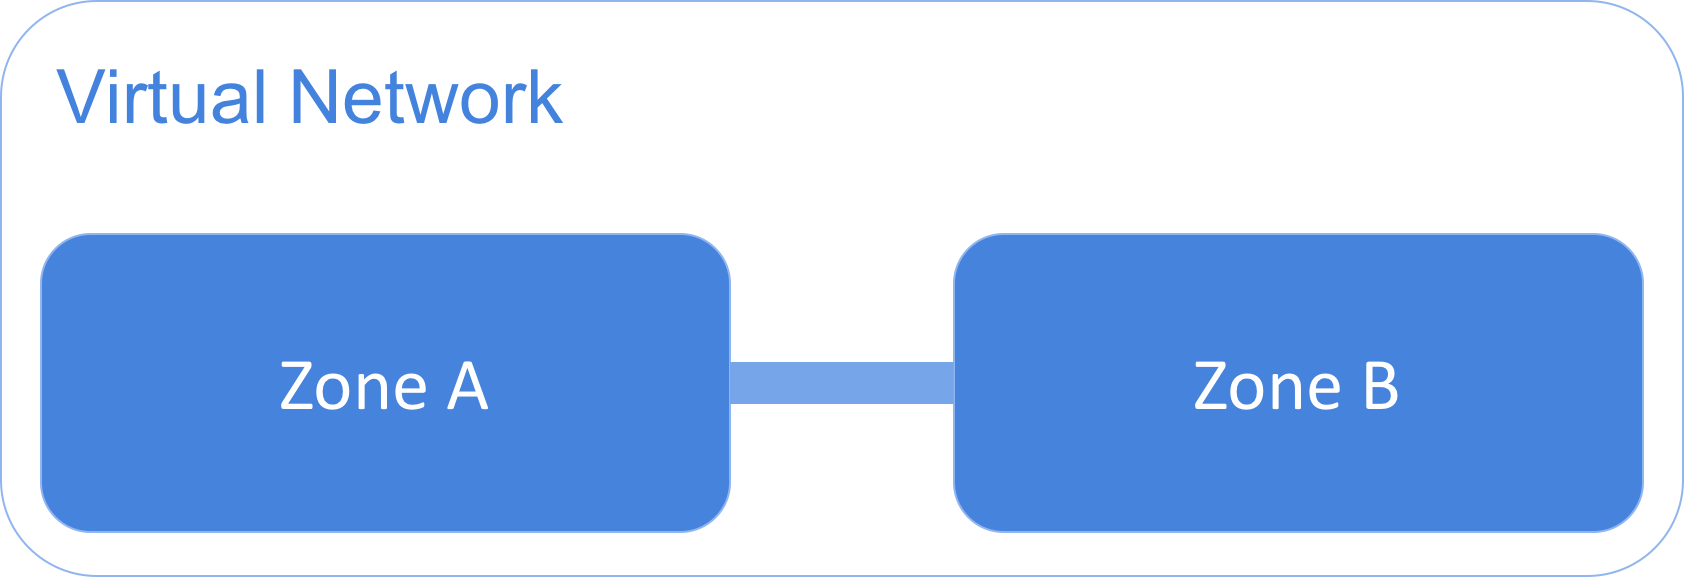
\includegraphics[width=1\textwidth]{images/system-nominal.png}
\end{figure}

During a \textbf{cluster crash}, a split brain scenario caused by the failure of either cluster, the remaining cluster can operate normally and execute all possible operations (shown in Figure \ref{fig:system-cluster-crash}).
In case the failed cluster is the secondary, the namenodes in the primary zone can continue without any modification to the behaviour but, if the failed cluster is the primary, the namenodes in the secondary zone require some adaptations.
Given that, in nominal operating conditions, namenodes in the secondary cluster execute all operations on the primary cluster, in case of failure of the primary zone a failover to the local cluster is required.
Once the primary cluster becomes available again, the secondary cluster invalidates all leases and both clusters wait for database replication to completely synchronize the primary zone with the secondary before allowing modifications again.
This process is necessary to guarantee that no conflicts are caused during transitions between states.
To summarize, in case of cluster crash the surviving cluster operates normally except for some contingencies during state transitions which are necessary to prevent conflicts.

\begin{figure}[h]
\caption{System during a cluster crash: one of the two clusters behaves normally while the other is unavailable.}
\label{fig:system-cluster-crash}
\centering
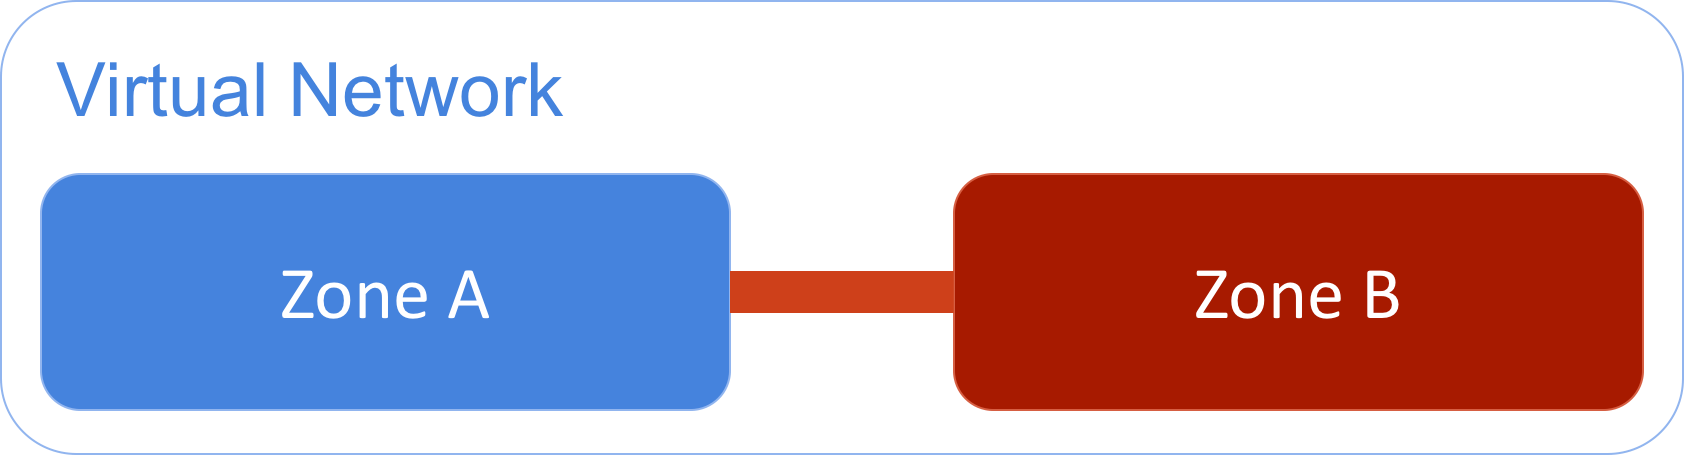
\includegraphics[width=1.0\textwidth]{images/system-cluster-crash.png}
\end{figure}

During a \textbf{network partition}, a situation where the two clusters function correctly but cannot communicate with each other as shown in Figure \ref{fig:system-network-partition}, concurrent modifications to metadata must be only allowed in such a way that prevents uncorrectable conflicts from happening.
To guarantee the absence of conflicts that cannot be automatically solved, the system in this state does not allow clients to perform a subset of metadata modifications.
More specifically, the only metadata modification allowed is the creation of new files and the subsequent append of data to such files, an operation for which automatic conflict resolution is possible in a deterministic fashion.
Any other operation is disallowed and an error is sent to the client attempting it.

\begin{figure}[h]
\caption{System during a network partition: both clusters are active but the connection between them has failed.}
\label{fig:system-network-partition}
\centering
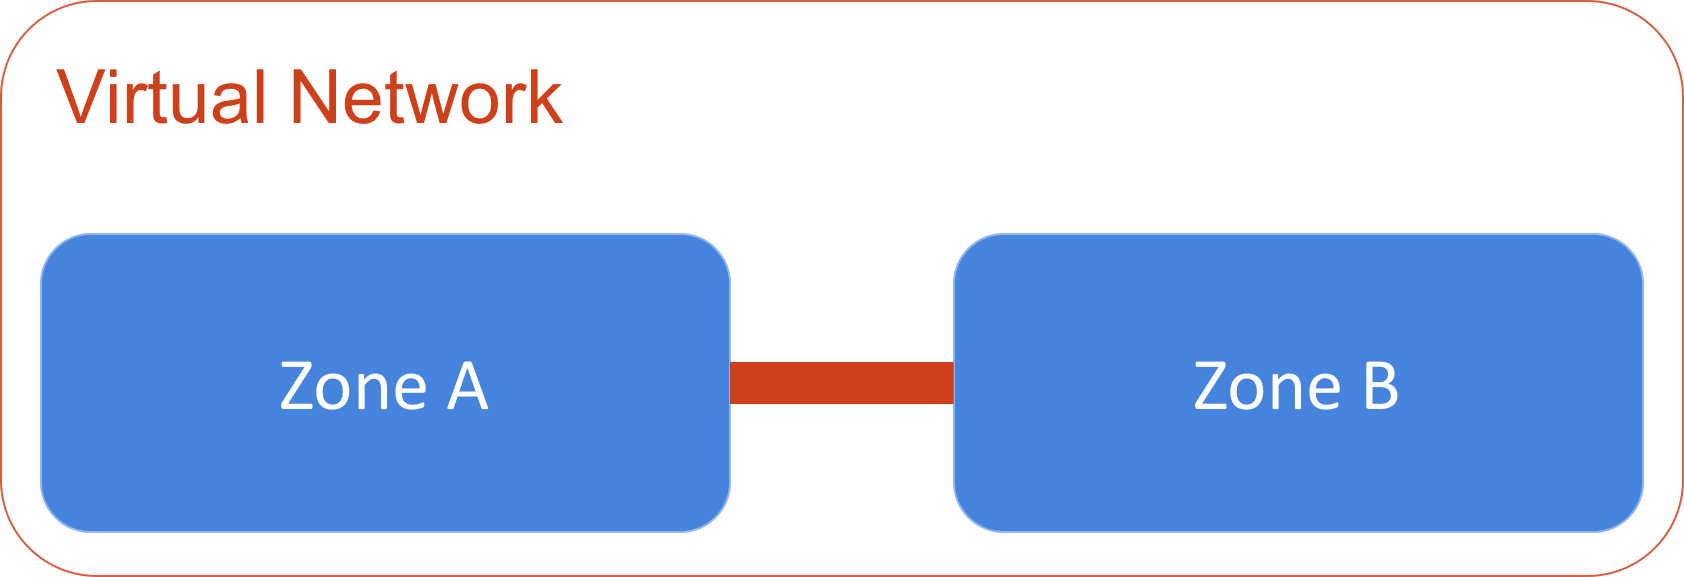
\includegraphics[width=1.0\textwidth]{images/system-network-partition.png}
\end{figure}

\subsubsection{Split brain detection}
In order to detect wheter the system is operating normally or it is suffering from a split brain we propose two different procedures, one for the primary and one for the secondary cluster, that allow namenodes to detect split brain scenarios with a minimum of internal coordination.
Coordination is provided by the leader election procedure described by Niazi et al \cite{DBLP:conf/fast/NiaziIHDGR17}, and discussed previously which is already present within HopsFS.

\paragraph{Detection on primary cluster}

To detect a split brain scenario on the primary cluster, we need to ascertain whether or not we are able to communicate with any node in the secondary cluster.
While we could implement a distributed failure detector to check for liveness of nodes in the secondary zone, HopsFS already exposes the failure detector built into the leader election procedure.
In the context of multiple data-centers, the leader election procedure is extended to include both namenodes from the primary and secondary cluster and a field in every row of the election table, to indicate the cluster the node belongs to.
Nodes from the secondary cluster connect directly to the primary cluster to perform leader election which means that, both in case of network partition and secondary cluster failure, the nodes would eventually be marked as not live by the failure detector.
With all of the prerequisites in place, the algorithm to detect network partitions on the primary cluster is illustrated in Algorithm \ref{algo:detection-primary}.

\begin{algorithm}[!ht]
	\begin{algorithmic}[1]
  		\caption{Split brain detection: primary cluster}
  		\label{algo:detection-primary}
  		\State $fd \leftarrow leaderElection$.getFD()
  		\Comment{get the failure detector from the leader election}
		\State $liveNodes \leftarrow fd$.getLiveNNSet()
		\For{$node$ in $liveNodes$}
		    \If{$node$.getCluster() == $\mathit{SECONDARY}$}
		        \State \Return $ok$
		    \EndIf
		\EndFor
		\State \Return $detected$
  	\end{algorithmic}
\end{algorithm}

\paragraph{Detection on secondary cluster}

The secondary cluster cannot rely on the same procedure as the primary cluster because, by definition, if a network partition happened or the primary cluster crashed, the connections of the namenodes to the primary clusters would be lost (and the leader election procedure would not run).
We can, however, treat the loss of connection as a signal that a network partition or cluster crash is occurring, but only if all nodes in the secondary cluster are not able to reach the primary.
One possible solution would be to have a table on the local database where namenodes write the status of their connection to the primary metadata cluster.
Given that namenodes can fail at any time, however, old entries from crashed nodes could actually result in false positives, impeding the other namenodes from detecting the partition.
In order to only query live namenodes we can use the same leader election component that we leverage in other parts of the system, running the algorithm on the local instance of NDB and only allowing local nodes to participate.
Instead of creating one extra table, we attach the status of the connection to the primary as a new column in the \emph{local} leader election instance.
With such a failure detector in place, detecting a split brain only requires checking the status of the connection to the primary on all other nodes, as shown in Algorithm \ref{algo:detection-secondary}.

\begin{algorithm}[!ht]
	\begin{algorithmic}[1]
  		\caption{Split brain detection: secondary cluster}
  		\label{algo:detection-secondary}
  		\If{$currentNode$.isConnectedToPrimary()}
  		    \State \Return $ok$
  		    \Comment{if the current node has a connection to the primary metadata cluster, there is no partition}
  		\EndIf
  		\Comment{get failure detector from leader election}
  		\State $fd \leftarrow secondaryLeaderElection$.getFD()
		\State $liveNodes \leftarrow fd$.getLiveNNSet() $\setminus \{currentNode\}$
		\For{$node$ in $liveNodes$}
		    \If{$node$.isConnectedToPrimary()}
		        \State \Return $ok$
		    \EndIf
		\EndFor
		\State \Return $detected$
  	\end{algorithmic}
\end{algorithm}

While namenodes are now capable of detecting a split brain independently, they don't have the capability of distinguishing between a network partition or a cluster crash.
This capability can be provided by providing a system hosted in a third zone, independent from the first two, which will act as a tie-breaker and allow the systems to consistently know whether both zones are still live (network partition) or if the remaining cluster is the only one currently running.
Such a system could be implemented in a variety of ways, for example by configuring a Zookeeper \cite{DBLP:conf/usenix/HuntKJR10} cluster with three nodes: one in the primary zone, one in the secondary zone and the tie-breaker in the third zone.
In case of split brain, both clusters would query the tie-breaking system which would yield one of the following outcomes:
\begin{enumerate}
    \item the cluster is unable to get a quorum of nodes; it is isolated both from the secondary and tie-breaker. In this case the cluster goes into read-only mode as it is the only safe course of action
    \item the cluster is able to get a quorum with the tie-breaker; the other cluster failed
    \item both clusters are able to contact the tie-breaker; the cluster is experiencing a network partition
\end{enumerate}

In case of cluster failure the remaining cluster can continue serving all requests from the clients.
The reason for this is because, following the tie-breaking, we are sure that the other cluster is either not live or in read mode, therefore there will be no conflicts upon restoring the asynchronous replication of metadata.
If the failed cluster is the primary, the secondary cluster namenodes need to switch over to the local cluster for write, as well as read operations, until such time where connectivity between the two clusters is restored and all necessary procedures to safely resume metadata replication have been executed.

While a cluster failure is relatively straightforward, network partition must be handled with extreme care to maintain the single-writer semantics of HDFS.
Should the two cluster be allowed to continue without any restrictions on the operations that they are allowed to perform, they could cause conflicts in such a way that required human intervention to merge.

\subsubsection{Conflict handling for network partitions}
Conflicts on file metadata can only happen in three classes of tables:
\begin{itemize}
    \item the inode table
    \item the block and replica tables
    \item the lease table
\end{itemize}.
While conflict on leases can be avoided by clearing the leases upon both detecting a partition and resolving the partition, forcing clients to retake the lease and retry the operation, conflicts on the inode and block tables must be handled.
\paragraph{Conflicts on block and replica tables} are particularly problematic as, after the partition is resolved, the system may be in a state where two disk blocks with different content have the same ID.
Upon replication, the metadata for the blocks created on the primary cluster would ``win'' and on-disk replicas created on the secondary cluster would therefore be considered corrupt on the first block report due to having a different checksum.
While it would be possible to devise a conflict resolution scheme to maintain both block versions, conflicts on blocks and replicas can be avoided altogether.
Before introducing the solution it is necessary to understand how ID assignment for blocks (and other database objects) is handled in HopsFS.
Given that \textit{addBlock} is a frequent operation when writing files doing a round-trip to the database to request each new block ID would be prohibitively slow and would create a large amount of work on the metadata cluster, this operation is batched.
At the first write operation, namenodes require a sequence (batch) of new IDs that they will use to fulfill subsequent \textit{addBlock} operations.
When all IDs in the batch have been assigned, the namenode just requests another batch.
By configuring the namenodes on the primary cluster to only require batches of \emph{even block IDs} and namenodes on the secondary cluster to require batches of \emph{odd block IDs}, two blocks created on two different clusters will never have the same block ID and will therefore never cause a conflict.

\paragraph{Conflicts on inodes,} on the other hand, are caused by both partitions creating a file or directory with the same name in the same parent directory.
As previously discussed, inodes also have unique IDs, but conflict are detected on the primary key which is composed of the name and parent ID. 
These conflicts are therefore unavoidable but they can be resolved with ease.
Upon detecting a conflict on the inode table, the inode created on the secondary cluster will be placed in the exception table due to the conflict resolution strategy.
With the inode in the exception table, the namenode responsible for handling conflicts (which is a leader elected between nodes in the primary cluster), can create a new inode with a different name and place it back in the same directory.
A possible example of such a naming scheme may be \texttt{<original name> + <sequential number>} such that if \texttt{myFolder/myFile} was created on both clusters, the conflicting file would be renamed as \texttt{myFolder/myFile\textbf{1}}.
Allowing files to sometimes be renamed is a significant difference in behaviour compared to both HDFS and HopsFS in single zone mode, which is why clients of the system need to take this behaviour into account and react to it upon resolution of a network partition.

By using the \emph{conflict avoidance and resolution} techniques developed, clients in both zones are allowed to continue all read and file creation operations with minor divergences in overall system behaviour.
The techniques presented, however, are only sufficient to handle the file creation case, but not other operations that require modification of metadata.
Given that in case of network partition the system doesn't have access to a consistent lease table, there is no way of knowing which existing files are being appended to, the only form of modification allowed on files in HDFS.
Allowing clients to append data to a file, could therefore result in two clusters having two diverging versions of the same block, a conflict which cannot be resolved without either creating two different copies of the file with new blocks or implementing a way for the system to handle diverging copies of the same file.
Due to the complexity both in terms of implementation and resulting behaviour of the proposed solutions, as well as the fact that in the Spotify synthetic workload shown in \cite{DBLP:conf/dais/NiaziIBD15} append operations account for 0.0\% of the total, the current course of action is to disallow them during network partition events.
Subtree operations, due to their use of locking and the large amount of transactions they generate, are also disallowed.
Deletes and moves are also not permitted due to the conflicts that they would generate.
This solution allows the two data-centers to operate independently during network partitions, albeit with a subset of operations.

A possible alternative for workloads that require the full set of operations is to implement an arbitration strategy similar to that used in NDB.
In this case, only one of the two sub-clusters would be allowed to continue performing write operations, while the other cluster would be free to continue in a read-only capacity.

\subsubsection{Summary}
In this section we describe a plan that allows the clusters to not only detect split brain situations, but to identify whether the situation is due to a network partition or a cluster crash and react accordingly.
While many operations are disallowed during network partitions, this should be a rare and transient event.
Furthermore this is only a plan for the initial implementation and restrictions may be lifted with further work on conflict resolution.

% \subsubsection{Representation}
% Metadata in HopsFS is managed by a relational database management system, and is therefore modelled as a number of independent tables containing data tuples known as rows.
% Each table has a fixed schema which defines the name and type of the elements contained in each tuple.
% Tables uniquely identify tuples according to their primary key, a user-defined subset of fields of the tuple itself.
% A primary key is unique for the table where is contained and this restriction is enforced by the database to maintain consistency.
% Primary keys are also instrumental to the conflict detection and resolution processes that are required to maintain the asynchronous system in a consistent state.
% Two transactions are considered conflicting if and only if they modify the same tuple as identified by primary key.
% 
% HopsFS stores the file system tree as inodes in the \emph{inode table}.
% Each inode is identified uniquely by its name and the unique id for the parent inode.
% Inodes are partitioned by NDB in such a way that all the children of any given inode are stored in the same shard, allowing for very fast directory listing.
% While directoryplit




\subsection{Block management}
Aside from managing metadata in a replicated environment, a geographically replicated storage system also needs to manage file content in such a way that, during a split brain, the separated clusters are capable of serving all client requests.
As previously mentioned, HDFS and HopsFS, store file content in \emph{blocks} which are managed by data nodes.
A file can span arbitrarily many blocks which have a configurable maximum size, by default 150 megabytes.
Blocks are immutable once they are marked as finished and only the last block in a file can be modified.
Adding content at the end of a block is the only modification allowed.

In order to maintain availability of blocks in the face of data node failure, HopsFS supports two different replication schemes: block replication and erasure coding.

\paragraph{In block replication,} the system maintains multiple copies of the same block on different data nodes.
The copies, called replicas, are distributed among data nodes according to a configurable placement policy, which aims to minimize the number of blocks which are unavailable as a result of component failure, be it machine or switch.
In case one of the replicas is permanently lost, the leader namenode instructs data nodes to re-replicate the block, returning the amount of replicas to the specified number, three by default.

\paragraph{Erasure coding} is a radically different concept than whole block replication.
Instead of creating entire copies of the blocks, erasure coding computes new parity blocks from the original blocks.
Both the number of source and output blocks are configurable, and the output blocks are called parity blocks.
Assuming $N$ source blocks, 10 for example, and $M$ parity blocks, 5 for example, the 10 original blocks can be reconstructed using any combination of the $N + M$ blocks now available.
The parity blocks form a new file, which is stored in a different directory than the original file.
Block placement for erasure coding blocks is handled by the \emph{erasure coding manager} which is described in \cite{grohsschmiedt2014making}.
In case one of the blocks for a erasure coded file fails, the system needs to regenerate either the original block or the parity block, which requires a full read of $N$ of the blocks and it is accomplished through a mapreduce job.

In this work we only consider whole block replication but we plan to implement erasure coding schemes in later iterations of the project.

\subsubsection{Placement policy}
Given that the goal for the project is to allow both geographical regions to operate independently in case of split brain, each region requires a complete set of blocks from all locations.
In order to obtain this, the block placement policy needs to be aware of the existence of multiple zones, which are considered separate failure domains.
The existing hierarchy for failure domains only considers machine and rack but the modified version will also include a third level: \emph{geographical zone}.

While this solves the issue of placing blocks in the correct datanodes, there remains the issue of the number of replicas to create.
The default value of three creates imbalance, by assigning two replicas in the zone where the block was created and only one in the other zone.
By using a replica value of four two replicas are assigned to every zone, ensuring that both zones have the same amount of blocks.

The final problem regarding the placement policy is the handling of split brain scenarios.
Without further adaptations, a split brain scenario would lead the cluster to believe that half of all the replicas in the cluster are missing, forcing the leader namenode to re-replicate all the blocks an additional two times.
Aside from creating a very large amount of network load between datanodes the result of such re-replication would be discarded as soon as the temporary split brain scenario is resolved.
In order to avoid spurious re-replication, we modify the amounts of replicas to two during split brain scenarios.
By setting the value to two, we avoid any re-replication of existing blocks and we only create two replicas for new blocks.
When the two clusters are merged, the replica value is once again increased to four, and the normal background re-replication tasks will create the necessary replicas in the other zone for blocks created during the split brain.

\subsubsection{}
\subsection{Adaptations}
As previously described in Section \ref{sec:dal}, the DAL was structured around access to a globally available connector, which in turn assumed a connection to a single cluster.
Due to these assumptions, the majority of the implementation work accomplished in the context of this thesis was to improve the DAL to allow multiple open connections to different databases.
Multiple database connections are necessary for the namenodes in the secondary cluster to route some queries to the local metadata storage cluster and some others to the primary cluster.
In addition to this, to be able to recover from network partitions, the DAL must be able to reconnect to the metadata storage cluster in case of failure and notify other components of this.
Notifications of disconnections and reconnections are necessary to correctly manage state changes for the system, namely enter and exit partition mode, both on the primary and on the secondary cluster.

\paragraph{Connection to multiple database}
As previously discussed, metadata accesses are not performed by directly accessing the connector but rather by using a request handler.
When operating on multiple databases there needs to be a mechanism for a request handler to be executed either on the local or the primary metadata cluster.
Note that a request for the local database still connects to the primary if the namenode requesting it is itself in the primary zone.
While a first implementation required every request handler to explicitly provide the database to connect to as a parameter this required modification of all code locations where a transaction handler is created.
This method is also extremely error prone as it disseminates the information on where to execute operations around the codebase.
The better solution is to associate to every operation type the database where the operation is to be executed.
This result is achieved by associating a constant to every member of the \texttt{OperationType} enumeration as shown in Listing \ref{lst:optype-enum}.
By extracting the database information from the \texttt{opType} the request handler can operate transparently without changes in signature and all the modifications are concentrated in one place, the operation type enumerator.

\begin{lstlisting}[label={lst:optype-enum}, caption={The OperationType enum}]
public interface OperationType {
    TransactionCluster getCluster();
} 

public enum HDFSOperationType implements OperationType {
    INITIALIZE(TransactionCluster.PRIMARY),
    ACTIVATE(TransactionCluster.PRIMARY),
    META_SAVE(TransactionCluster.PRIMARY),
    SET_PERMISSION(TransactionCluster.PRIMARY),
    SET_OWNER(TransactionCluster.PRIMARY),
    SET_OWNER_SUBTREE(TransactionCluster.PRIMARY),
    GET_BLOCK_LOCATIONS(TransactionCluster.PRIMARY),
    GET_STATS(TransactionCluster.PRIMARY),
    CONCAT(TransactionCluster.PRIMARY),
    // many more

    private TransactionCluster cluster;

    HDFSOperationType(TransactionCluster c) {
        this.cluster = c;
    }

    private TransactionCluster getCluster() {
        return this.cluster;
    }
}
\end{lstlisting}

Request handlers obtain a connector to a specific database using a \emph{multizone storage connector}, shown in Listing \ref{lst:multizone-connector} along with .
This interface, which is implemented both in the primary cluster and in the secondary cluster, allows clients to obtain a concrete connector towards a single database.
In future iterations of the project, the multizone connector will also modify its behaviour during network partitions, for instance by always returning the local connector on the secondary cluster during a cluster crash.
\begin{lstlisting}[label={lst:multizone-connector}, caption={The MultiZoneStorageConnector interface}]
/**
 * This class allows its clients to retrieve a connector 
 * for the required cluster (primary or local).
 */
public interface MultiZoneStorageConnector {
  /**
   * This method returns a StorageConnector
   * for the appropriate cluster.
   * @param cluster whether to connect to
   * the local or primary cluster
   * @return the appropriate storage connector
   * @throws StorageException if a connector
   * cannot be returned
   */
  StorageConnector connectorFor(TransactionCluster cluster)
    throws StorageException;
}
\end{lstlisting}

The database connector was also modified to allow for re-connection capabilities and notifications of changes in state by implementing the \texttt{Reconnector} interface shown in Listing \ref{lst:reconnector}.
The information on whether the connection is functioning or not is used on the secondary cluster by a \texttt{partition monitor} to perform split brain detection as shown in Algorithm \ref{algo:detection-secondary} and Listing \ref{lst:detection-secondary}.
When a split brain is detected by a partition monitor, a configurable action is executed and this action will, in the future, perform the state changes required by the system to handle the partition.
\begin{lstlisting}[caption={Implementation of the partition detection algorithm in the secondary cluster}, label={lst:detection-secondary}]
/**
 * This methods performs partition detection
 * for the secondary cluster.
 * A partition is detected in the secondary cluster if all
 * the live namenodes lost the connection
 * to the primary cluster.
 * Additionally, this class updates the state 
 * of the node's connection in the leader election procedure.
 */
@Override
protected PartitionEvent tick() {
    boolean connected = connector.isConnectedToPrimary();

    // update the state of the connection
    // in the leader election procedure
    leaderElection.setConnectedToPrimary(connected);
    // if connected to primary there is at least
    // one node connected (therefore no partition).
    if (connected) {
        return PartitionEvent.RESOLVED;
    }

    // if at least one of the other nodes is connected,
    // the partition is resolved.
    SortedActiveNodeList namenodes = 
        leaderElection.getActiveNamenodes();
    // this can happen if run before the first leader 
    // election round. unknown is ignored
    if (namenodes == null) {
        return PartitionEvent.UNKNOWN;
    }
    for (ActiveNode n: namenodes.getActiveNodes()) {
        if (n.isConnectedToPrimary()) {
            return PartitionEvent.RESOLVED;
        }
    }

    // if all the active namenodes aren't connected
    // to the database, detect a partition.
    return PartitionEvent.DETECTED;
}
\end{lstlisting}

\begin{lstlisting}[caption={Reconnector interface}, label={lst:reconnector}]
/**
 * A reconnector can report whether the 
 * connection is up and attempt reconnections.
 * Note that, if possible, checking
 * for connectivity should be cheap while
 * reconnection is expected to be more expensive.
 */
public interface Reconnector {
  /**
   * Checks whether the connector is connected to the remote.
   * @return whether the connection is up
   */
  boolean isConnected();

  /**
   * Attempts a reconnection.
   * If this method returns successfully,
   * the connection attempt was a success.
   * Should be called periodically
   * in the background to re-acquire connectivity
   */
  void reconnect() throws StorageException;
}
\end{lstlisting}

While the work performed so far is necessary to allow further progress towards the implementation of the theoritical framework described in this chapter, there is still much to do.
The distinction between network partition and cluster crash is not implemented and will require an external system like ZooKeeper to perform arbitration.
The routing of operations to the local database and all of the changes to the client to allow it to perform fully consistent reads are not implemented.
Finally the behaviour of the system will need to be tested to make sure that it conforms with the expected behaviour described.

\clearpage

\section{Summary} 
\label{sec:summary}
In this work we present a solution that allows HopsFS to transparently present multiple geographical areas as one cluster to clients.
By leveraging the asynchronous replication built into MySQL cluster we perform metadata replication across geographical areas while still maintaining the same consistency guarantees as Apache HDFS and HopsFS when deployed in a single area.
We also describe solutions for both network partitions and cluster crashes which allows clients to continue performing a safe subset of operations and allows the system to recover gracefully from such events.
Furthermore, we detail the implementation work done to allow the inclusion of such changes into the HopsFS codebase.
To the best of our knowlege, once complete, this would be the first HDFS implementation with such characteristics allowing it to reach the same levels of availability and data retention as cloud native storage systems such as Amazon S3, while still maintaining the consistent behaviour of a hierarchical file-system.
\subsection{Future work}
While the description of the basic solution presented in this thesis is complete, there is still much to be done both to implement the basic solution in the code and to further optimize it.
Specifically, the implementation work done so far only covers the adaptation of the metadata access layer (DAL) to allow it to connect to multiple database clusters at the same time as well as being able to detect disconnections and perform re-connections.
Futhermore, while the conflict detection functions used to merge the system after a network partition are provided by MySQL Cluster, no testing was perfomed regarding their impact on the performance of the database.
There are also several areas where the proposed solution could be improved.
First of, it would be interesting to study a way to execute some operations on the local cluster instead of routing them all to the primary cluster, while still maintaining the same consistency guarantees.
By doing that we would further reduce the strain on the primary cluster and increase scalability of the overall system.
Similarly, it would be beneficial to allow a greater set of operations when the cluster is experiencing a network partition to increase compatibility with applications that expect Apache HDFS and are therefore unaware of multiple zones.
Finally, there are several key improvements to consider in the context of block storage and replication.
Erasure coding techniques \cite{DBLP:conf/usenix/HuangSXOCG0Y12,grohsschmiedt2014making} can reduce the block replication overhead allowing better utilization of space in the cluster, while improvements in block placement policies (as shown in \cite{DBLP:conf/usenix/CidonRSKOR13}) can dramatically increase data retention in the presence of failures.
\clearpage

%% The \phantomsection command is nessesary for hyperref to jump to the 
%% correct page, in other words it puts a hyper marker on the page.

\phantomsection

\bibliographystyle{abbrv}
\bibliography{biblio}

%% Appendices
%% Liitteet
% \clearpage
% 
% \thesisappendix
% 
% \section{Esimerkki liitteest\"a\label{LiiteA}}
% 
% Liitteet eiv\"at ole opinn\"aytteen kannalta v\"altt\"am\"att\"omi\"a ja 
% opinn\"aytteen tekij\"an on 
% kirjoittamaan ryhtyess\"a\"an hyv\"a ajatella p\"arj\"a\"av\"ans\"a ilman liitteit\"a.
% Kokemattomat kirjoittajat, jotka ovat huolissaan
% tekstiosan pituudesta, paisuttavat turhan 
% helposti liitteit\"a pit\"a\"akseen tekstiosan pituuden annetuissa rajoissa.
% T\"all\"a tavalla ei synny hyv\"a\"a opinn\"aytett\"a.   
% 
% Liite on itsen\"ainen kokonaisuus, vaikka se t\"aydent\"a\"akin tekstiosaa.
% Liite ei siten ole pelkk\"a listaus, kuva tai taulukko, vaan 
% liitteess\"a selitet\"a\"an aina sis\"all\"on laatu ja tarkoitus. 
% 
% Liitteeseen voi laittaa esimerkiksi listauksia. Alla on 
% listausesimerkki t\"am\"an liitteen luomisesta. 
% 
% %% Verbatim-ymp\"arist\"o ei muotoile tai tavuta teksti\"a. Fontti on monospace.
% %% Verbatim-ymp\"arist\"on sis\"all\"a annettuja komentoja ei LaTeX k\"asittele. 
% %% Vasta \end{verbatim}-komennon j\"alkeen jatketaan k\"asittely\"a.
% \begin{verbatim}
% 	\clearpage
% 	\appendix
% 	\addcontentsline{toc}{section}{Liite A}
% 	\section*{Liite A}
% 	...
% 	\thispagestyle{empty}
% 	...
% 	teksti\"a
% 	...
% 	\clearpage
% \end{verbatim}
% 
% Kaavojen numerointi muodostaa liitteiss\"a oman kokonaisuutensa:
% \begin{eqnarray}
% d \wedge A  &=& F, \label{liitekaava1}\\
% d \wedge F  &=& 0. \label{liitekaava2}
% \end{eqnarray}
% 
% 
% \clearpage
% \section{Toinen esimerkki liitteest\"a\label{LiiteB}}
% 
% %% Liitteiden kaavat, taulukot ja kuvat numeroidaan omana kokonaisuutenaan
% %%
% %% Equations, tables and figures have their own numbering in Appendices
% %\renewcommand{\theequation}{B\arabic{equation}}
% %\setcounter{equation}{0}  
% %\renewcommand{\thefigure}{B\arabic{figure}}
% %\setcounter{figure}{0}
% %\renewcommand{\thetable}{B\arabic{table}}
% %\setcounter{table}{0}
% 
% Liitteiss\"a voi my\"os olla kuvia, jotka
% eiv\"at sovi leip\"atekstin joukkoon:
% %% Ymp\"arist\"on figure parametrit htb pakottavat
% %% kuvan t\"ah\"an, eik\"a LaTeX yrit\"a siirrell\"a niit\"a
% %% hyv\"aksi katsomaansa paikkaan. 
% %% Ymp\"arist\"o\"a center voi k\"aytt\"a\"a \centering-
% %% komennon sijaan
% %%
% %% Example of a figure, note the use of htb parameters which force
% %% the figure to be inserted here
% \begin{figure}[htb]
% \begin{center}
% 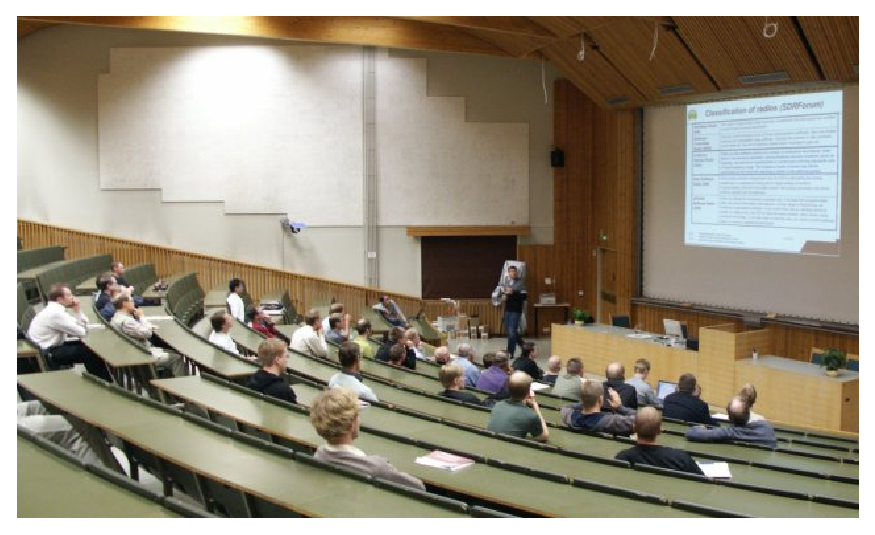
\includegraphics[height=8cm]{kuva2}
% \end{center}
% \caption{Kuvateksti, jossa on liitteen numerointi}
% \label{liitekuva}
% \end{figure}
% %%
% Liitteiden taulukoiden numerointi on kuvien ja kaavojen kaltainen:
% \begin{table}[htb]
% \caption{Taulukon kuvateksti.}
% \label{liitetaulukko}
% \begin{center}
% \fbox{
% \begin{tabular}{lp{0.5\linewidth}}
% 9.00--9.55  & K\"aytett\"avyystestauksen tiedotustilaisuus (osanottajat
% ovat saaneet s\"ahk\"opostitse valmistautumisteht\"av\"at, joten tiedotustilaisuus
% voidaan pit\"a\"a lyhyen\"a).\\
% 9.55--10.00 & Testausalueelle siirtyminen
% \end{tabular}}
% \end{center}
% \end{table}
% Kaavojen numerointi muodostaa liitteiss\"a oman kokonaisuutensa:
% \begin{eqnarray}
% T_{ik} &=& -p g_{ik} + w u_i u_k + \tau_{ik},  \label{liitekaava3} \\
% n_i    &=& n u_i + v_i.                      \label{liitekaava4}
% \end{eqnarray}
% 
\end{document}
% 